% ===========================================================================
% Results
% File: sections/04_results.tex
% Built sub-section by sub-section
% ===========================================================================

\section{Results}
\label{sec:results}

% ---------------------------------------------------------------------------

% ---------------------------------------------------------------------------
\subsection{Optimization Convergence and Optimal Design Parameters}
\label{sec:results_optimal}
% ---------------------------------------------------------------------------

\hspace{1cm}The Differential Evolution optimizer converged to feasible
solutions within 50 generations at all four sites. Runtime ranged from
102\,s (Konya) to 172\,s (Ouagadougou) on a standard desktop CPU,
reflecting differences in feasibility constraint violation frequency
across the population during early generations. The convergence curves
(Figure~\ref{fig:convergence}) show rapid improvement in the first
10--15 generations followed by progressive refinement, with no evidence
of premature convergence or stagnation.

\begin{figure}[H]
	\centering
	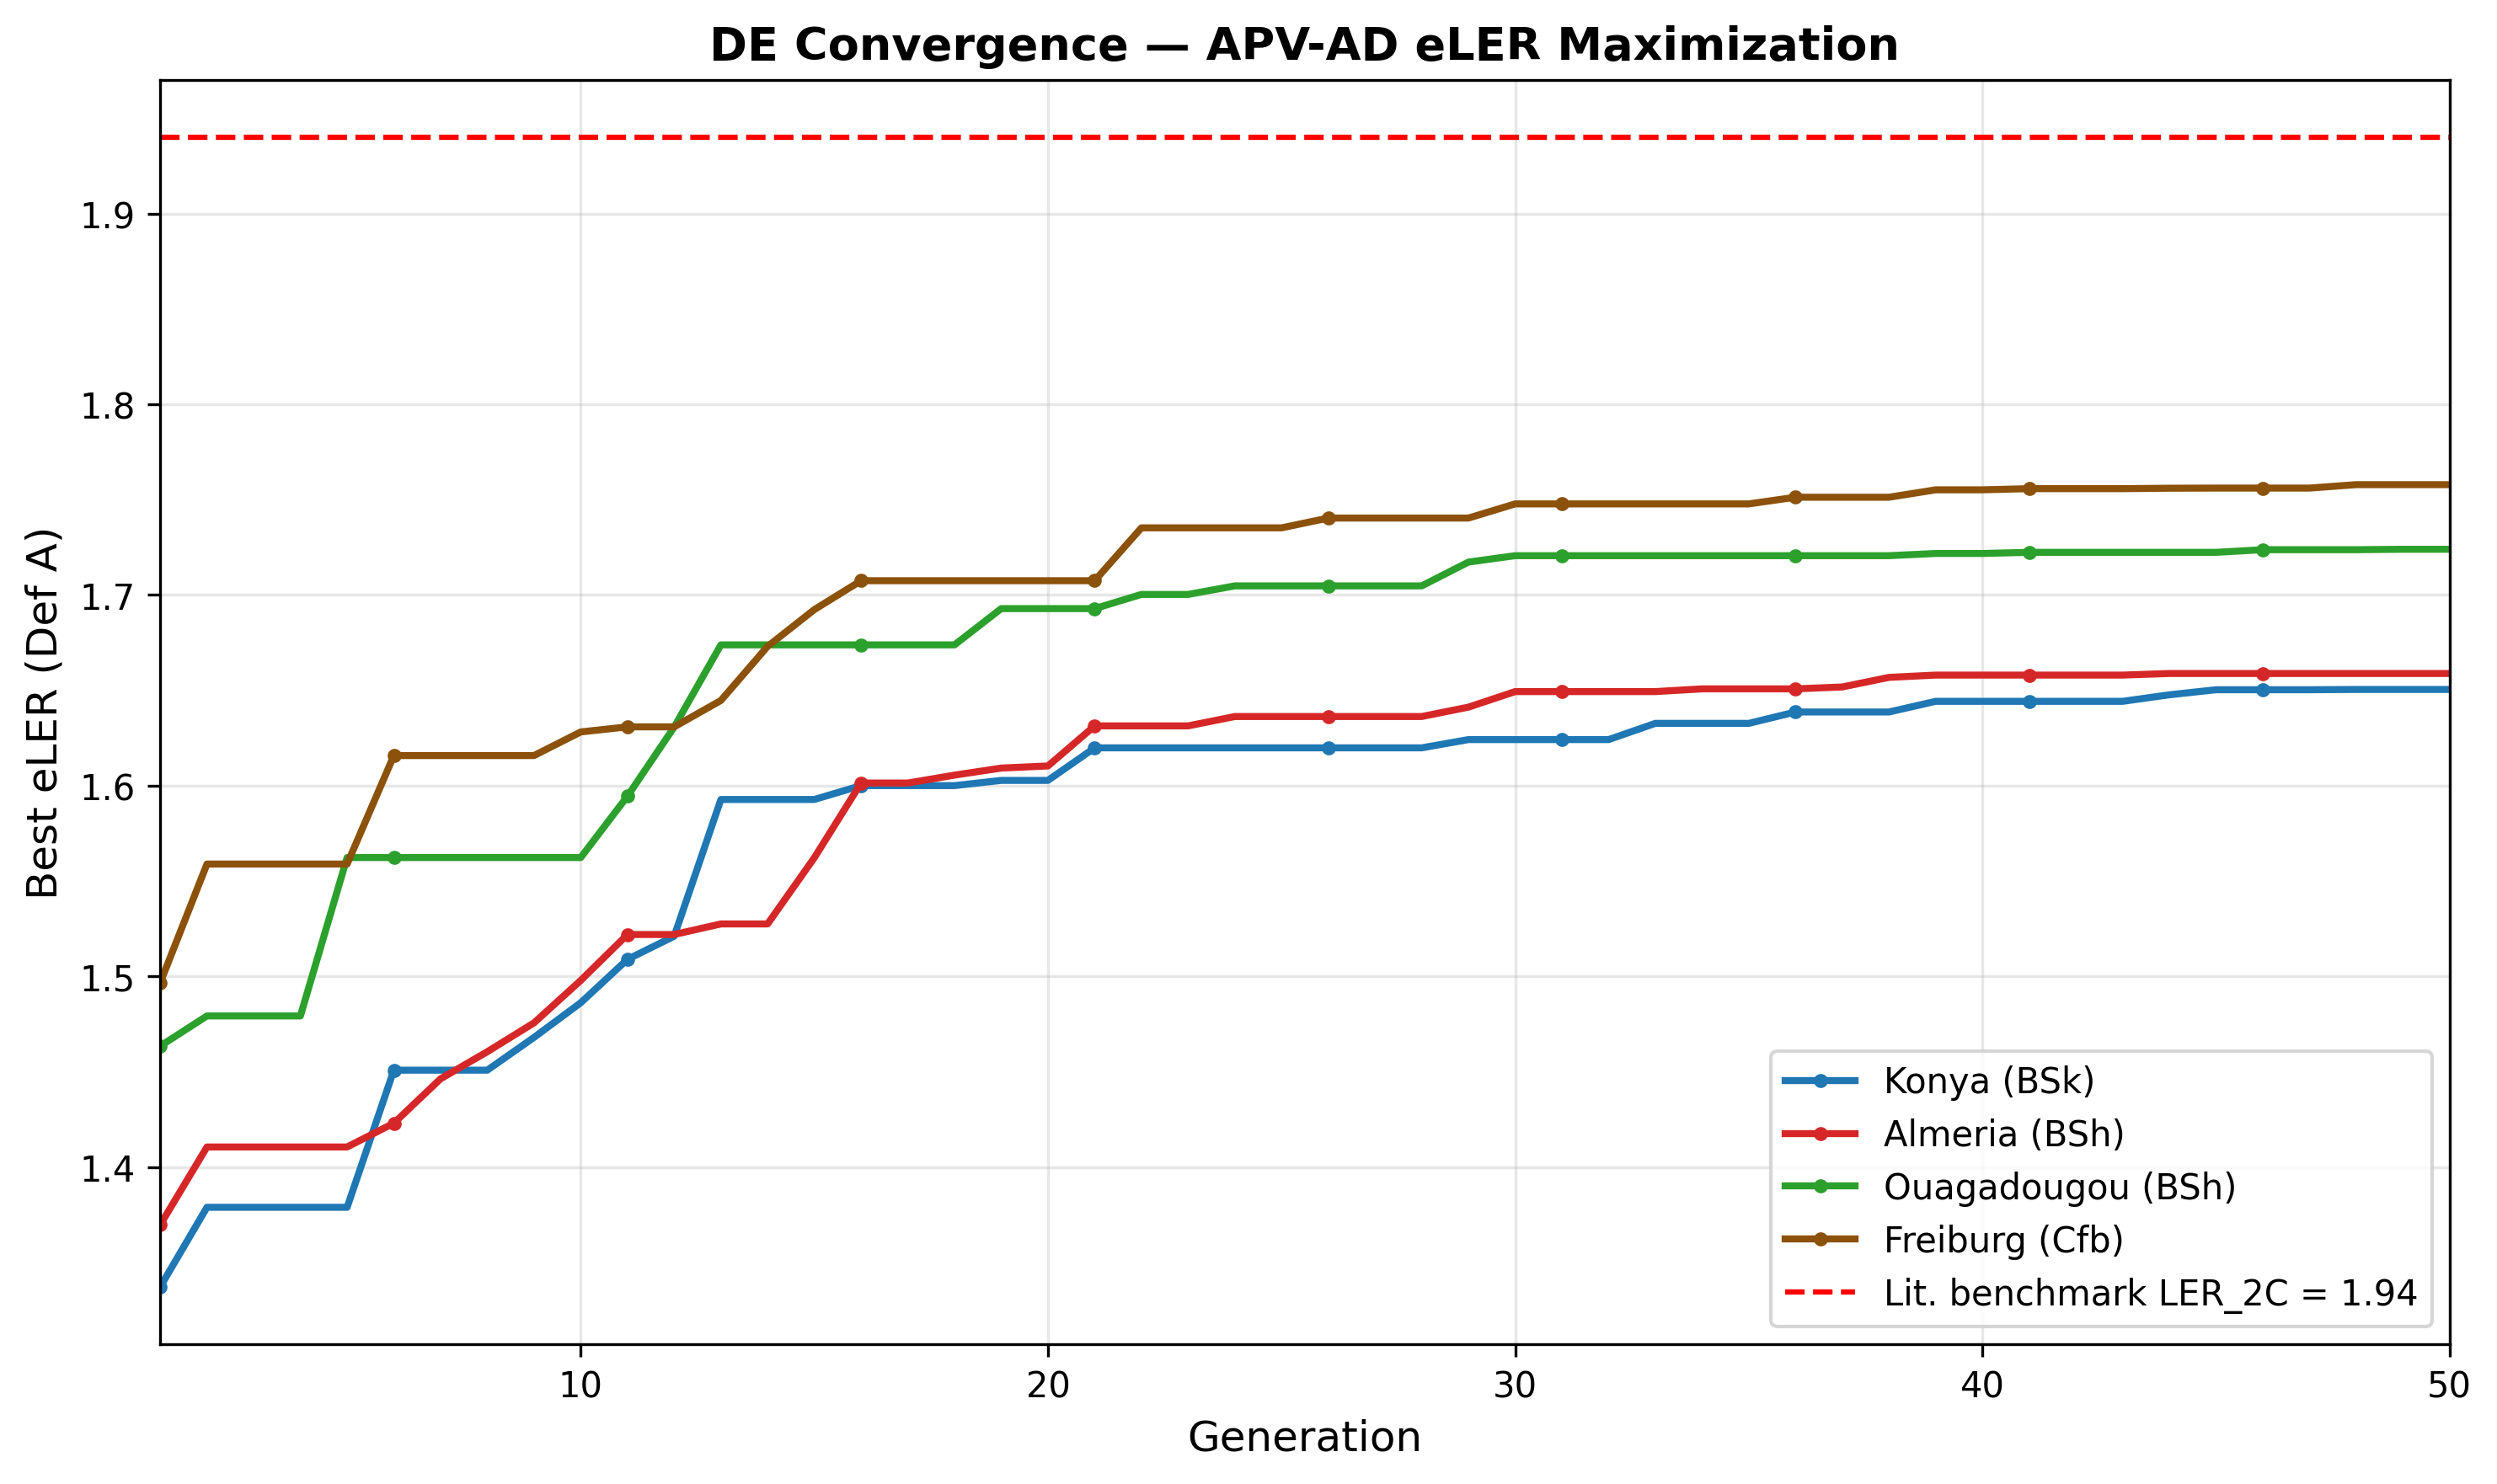
\includegraphics[width=\textwidth]{figures/fig_convergence.png}
	\caption{DE convergence curves for all four sites: best eLER (Definition~A)
		as a function of generation number. The red dashed line indicates the
		published two-component LER benchmark of 1.94~\citep{riaz2022}. All
		sites exceed this benchmark when the biogas term is included.}
	\label{fig:convergence}
\end{figure}

Table~\ref{tab:optimal} reports the optimal design variables and
primary performance metrics for all four sites after L-BFGS-B polishing.

\begin{table}[H]
	\caption{Optimal design parameters and primary performance metrics
		for all four sites (Scenario S0, baseline). All values correspond
		to the L-BFGS-B-polished DE solution.}
	\label{tab:optimal}
	\centering
	\begin{tabular}{lcccc}
		\toprule
		\textbf{Parameter} & \textbf{Konya} & \textbf{Almer\'{i}a}
		& \textbf{Ouagadougou} & \textbf{Freiburg} \\
		\midrule
		Tilt angle $\beta^*$ (°)       & 20.1  & 20.9  & 16.0  & 22.9  \\
		Row spacing $d_{\text{row}}^*$ (m) & 3.03 & 3.03 & 3.03 & 3.03 \\
		Module height $H_m^*$ (m)      & 1.50  & 1.50  & 1.50  & 1.50  \\
		Digester volume $V_{\text{dig}}^*$ (m³) & 3.64 & 4.14 & 3.52 & 3.10 \\
		HRT$^*$ (days)                 & 23.3  & 30.8  & 28.3  & 27.5  \\
		$f_{\text{PV,heat}}^*$         & 0.051 & 0.051 & 0.050 & 0.051 \\
		GCR (\%)                       & 70.6  & 70.2  & 72.3  & 69.3  \\
		OLR (kg\,VS\,m$^{-3}$\,d$^{-1}$) & 1.88 & 1.65 & 2.00 & 1.82 \\
		\bottomrule
	\end{tabular}
\end{table}

Three structural findings emerge from Table~\ref{tab:optimal}.

\textbf{Finding 1 --- Boundary convergence on row spacing and module
	height.} The optimizer converges to $d_{\text{row}}^* = \SI{3.03}{m}$
at all four sites --- the minimum value permitted by the inter-row
clearance constraint (Equation~\ref{eq:overlap}) at the optimal tilt
angles of 16--23°. Similarly, $H_m^* = \SI{1.50}{m}$ at all sites,
the specified lower bound. This boundary convergence indicates that
the eLER landscape has its global maximum at the physical constraint
boundary: increasing panel density simultaneously raises
$E_{\text{PV,sold}}$ (more modules per hectare) and increases
$F_{\text{shad}}$ (reducing $PAR_{\text{open}}$ denominator in
Equation~\ref{eq:lercrop}), both of which improve eLER. The
L-BFGS-B polishing step confirms that no interior local maximum
exists in the neighbourhood of the boundary solution. The eLER
penalty associated with any mechanical access corridor beyond the
minimum physical clearance is discussed in
Section~\ref{sec:discussion}.

\textbf{Finding 2 --- Climate-specific tilt angles.} Unlike row
spacing and module height, the optimal tilt angle varies meaningfully
across sites: from $\beta^* = 16.0$° at Ouagadougou (12.37°N, low
latitude) to $\beta^* = 22.9$° at Freiburg (47.99°N, high latitude).
This variation reflects the trade-off between maximising annual PV
yield (which favours a tilt closer to the site latitude) and
minimising the inter-row shading shadow length (which favours a
lower tilt at a given $d_{\text{row}}$). The optimal tilt is
approximately 0.4--0.5 times the site latitude, consistent with
the latitude rule-of-thumb for fixed-tilt systems but modified
downward by the shading penalty.

\textbf{Finding 3 --- Small digester volumes.} Optimal digester
volumes of 3.10--4.14\,m³ reflect the modest VS input from
1\,ha of tomato cultivation combined with cattle manure co-substrate
(VS$_{\text{total}}$ = 1\,892--2\,573\,kg\,ha$^{-1}$\,yr$^{-1}$).
OLR values of 1.65--2.00\,kg\,VS\,m$^{-3}$\,d$^{-1}$ are within
the stable mesophilic operating range $[1.5,\,5.0]$ at all sites,
confirming feasibility. The minimum heating fraction
$f_{\text{PV,heat}}^* \approx 0.05$ at all sites confirms that
the PV array provides far more energy than the digester requires:
5\% of annual PV output is more than sufficient to cover all
thermal demand.

% ---------------------------------------------------------------------------
\subsection{Extended Land Equivalent Ratio Decomposition}
\label{sec:results_eler}
% ---------------------------------------------------------------------------

\hspace{1cm}Table~\ref{tab:eLER} presents the complete eLER decomposition
for all four sites under Scenario S0 (baseline). Figure~\ref{fig:eler}
displays the same results as a stacked bar chart, enabling direct visual
comparison of the three components across sites and reference definitions.

\begin{table}[H]
	\caption{eLER decomposition for all four sites (Scenario S0, baseline).
		Definition~A uses an independent dense-pack PV reference;
		Definition~B uses GCR as the PV reference (circular).
		Literature benchmark: maximum two-component LER of 1.94
		from \citet{riaz2022}.}
	\label{tab:eLER}
	\centering
	\begin{tabular}{lcccc}
		\toprule
		\textbf{Metric} & \textbf{Konya} & \textbf{Almer\'{i}a}
		& \textbf{Ouagadougou} & \textbf{Freiburg} \\
		\midrule
		$LER_{\text{crop}}$                  & 0.363 & 0.367 & 0.397 & 0.371 \\
		$LER_{\text{PV}}$ (Def.~A)           & 0.675 & 0.676 & 0.691 & 0.660 \\
		$LER_{\text{PV}}$ (Def.~B = GCR)     & 0.706 & 0.703 & 0.723 & 0.693 \\
		$LER_{\text{biogas}}$                & 0.615 & 0.617 & 0.636 & 0.727 \\
		\midrule
		\textbf{eLER (Def.~A)}               & \textbf{1.653} & \textbf{1.659}
		& \textbf{1.725} & \textbf{1.758} \\
		eLER (Def.~B)                        & 1.684 & 1.686 & 1.756 & 1.791 \\
		$LER_{\text{2C}}$ (Def.~A)           & 1.038 & 1.042 & 1.089 & 1.031 \\
		Lit. benchmark $LER_{\text{2C}}$     & \multicolumn{4}{c}{1.94~\citep{riaz2022}} \\
		\bottomrule
	\end{tabular}
\end{table}

\begin{figure}[H]
	\centering
	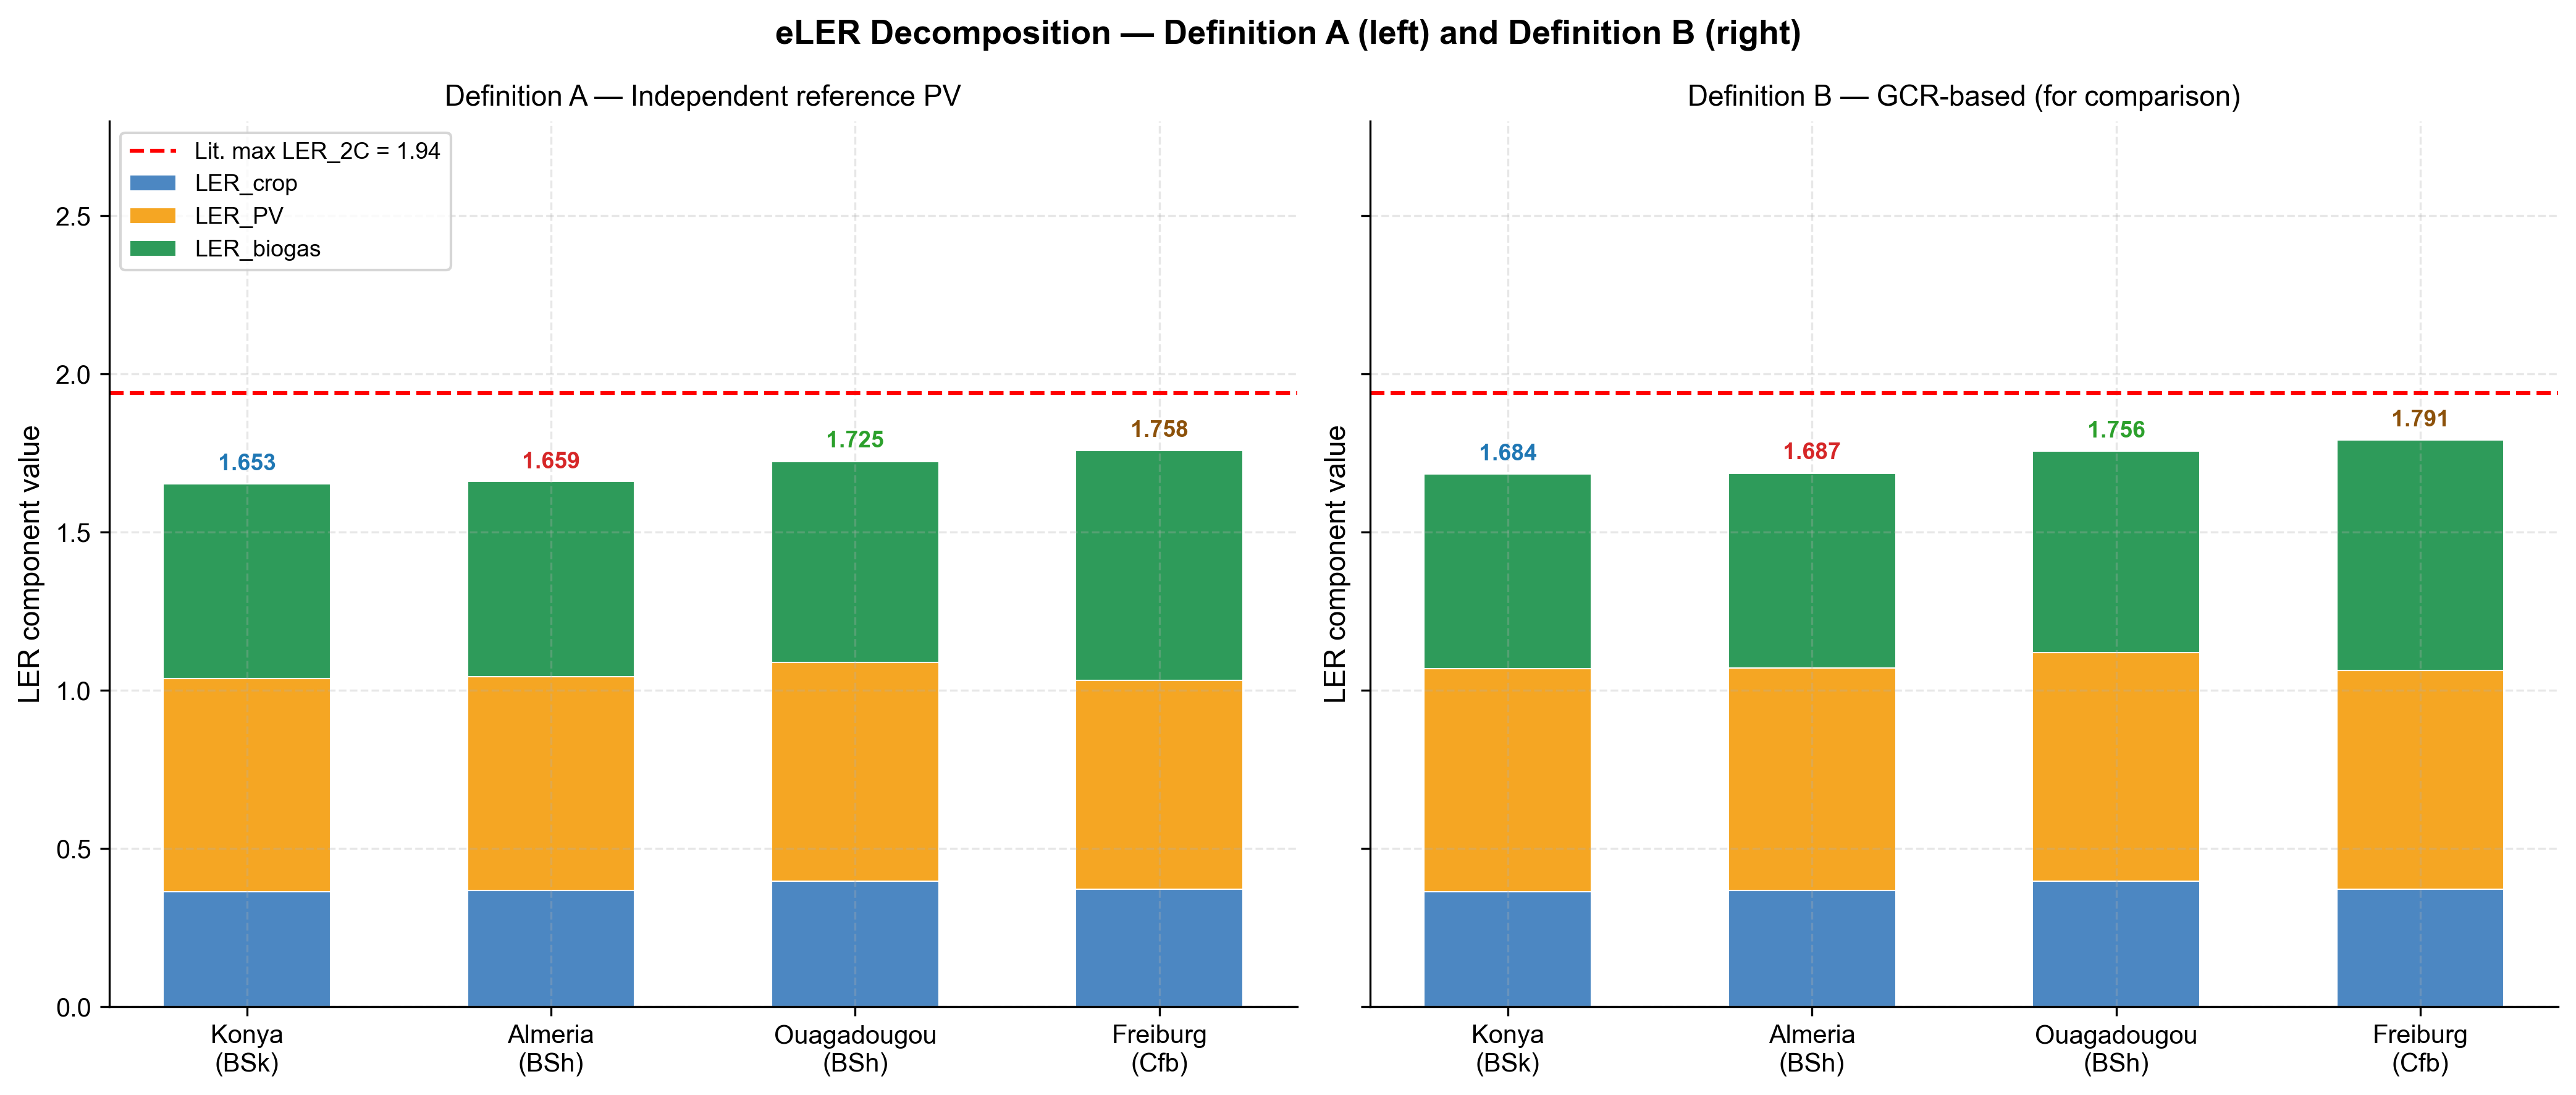
\includegraphics[width=\textwidth]{figures/fig03_eLER_stacked.png}
	\caption{eLER decomposition stacked bar chart for all four sites.
		Left panel: Definition~A (independent PV reference); right panel:
		Definition~B (GCR-based, circular). Blue: $LER_{\text{crop}}$;
		orange: $LER_{\text{PV}}$; green: $LER_{\text{biogas}}$. Red dashed
		line: published two-component maximum LER$_{\text{2C}}$ = 1.94
		\citep{riaz2022}. Annotated values are eLER totals (Definition~A).}
	\label{fig:eler}
\end{figure}

Three findings emerge from the eLER decomposition.

\textbf{Finding 1 --- $LER_{\text{2C}} > 1.0$ at all sites.}
The two-component agrivoltaic LER (crop + PV, without biogas) ranges
from 1.031 (Freiburg) to 1.089 (Ouagadougou), confirming that the
APV system outperforms two separate monocultures at every site even
without the AD contribution. This result improves on the $LER_{\text{2C}}$
reported in earlier versions of the model and reflects the boundary
convergence to high GCR (69--72\%), which substantially increases
$LER_{\text{PV}}$ relative to lower-density designs. However,
$LER_{\text{2C}}$ remains well below the published benchmark of 1.94
at all sites, confirming that the biogas term is the primary driver of
the eLER advantage over the two-component benchmark.

\textbf{Finding 2 --- $LER_{\text{biogas}} < 1.0$ at all sites.}
$LER_{\text{biogas}}$ ranges from 0.615 (Konya) to 0.727 (Freiburg),
meaning the APV--AD system produces less biogas than the standalone
open-field reference AD unit. This is a structural consequence of
the shading-residue coupling: with $LER_{\text{crop}} \approx 0.36$--$0.40$,
the APV system produces only 36--40\% of the open-field crop residue
quantity, reducing VS$_{\text{residues}}$ input to the digester
proportionally. The manure co-substrate ($VS_{\text{manure}}$),
identical in both the APV and reference cases, partially compensates
for this deficit, raising $LER_{\text{biogas}}$ above the value it
would take under residues-only digestion. Freiburg achieves the
highest $LER_{\text{biogas}}$ (0.727) because its lower open-field
reference yield (30\,t\,ha$^{-1}$ vs.\ 60\,t\,ha$^{-1}$ at other
sites) reduces the reference VS input, making the APV/reference
biogas ratio more favourable.

\textbf{Finding 3 --- $LER_{\text{PV}}$ is near-uniform across sites
	despite 1.8$\times$ GHI variation.}
$LER_{\text{PV}}$ (Definition~A) ranges narrowly from 0.660 (Freiburg)
to 0.691 (Ouagadougou), despite annual GHI varying from
1\,150 to 2\,050\,kWh\,m$^{-2}$. This uniformity arises because
Definition~A references a dense-pack array at the same tilt angle
$\beta^*$: both the APV system and the reference are subject to the
same local irradiance, and their ratio reflects only the shading
loss within the APV array. Since GCR is near-identical at all sites
(69--72\%) due to boundary convergence, the inter-row shading pattern
--- and hence $LER_{\text{PV}}$ --- is also near-identical. The small
variation across sites reflects differences in solar elevation angle
distribution, which modulates the effective shading fraction at a
given GCR.

% ---------------------------------------------------------------------------
\subsection{Energy Performance and Thermal Balance}
\label{sec:results_energy}
% ---------------------------------------------------------------------------

\hspace{1cm}Table~\ref{tab:energy} summarises annual energy performance
for all four sites. Figure~\ref{fig:energy} presents the monthly energy
balance, showing the seasonal distribution of PV generation, biogas
production, and digester heat demand.

\begin{table}[H]
	\caption{Annual energy performance and thermal balance for all four
		sites (Scenario S0, 1\,ha normalisation).}
	\label{tab:energy}
	\centering
	\begin{tabular}{lcccc}
		\toprule
		\textbf{Parameter} & \textbf{Konya} & \textbf{Almer\'{i}a}
		& \textbf{Ouagadougou} & \textbf{Freiburg} \\
		\midrule
		PV total (MWh\,ha$^{-1}$\,yr$^{-1}$)    & 1\,354 & 1\,577 & 1\,583 & 1\,108 \\
		PV sold to grid (MWh\,ha$^{-1}$\,yr$^{-1}$) & 1\,286 & 1\,498 & 1\,503 & 1\,052 \\
		PV self-consumed (MWh\,ha$^{-1}$\,yr$^{-1}$) & 68 & 79 & 80 & 56 \\
		Biogas total (MWh\,ha$^{-1}$\,yr$^{-1}$) & 3.68 & 3.83 & 5.99 & 2.87 \\
		Heat demand (MWh\,ha$^{-1}$\,yr$^{-1}$)  & 1.92 & 1.54 & 1.12 & 2.08 \\
		Biogas for heating (MWh\,ha$^{-1}$\,yr$^{-1}$) & 0.00 & 0.00 & 0.00 & 0.00 \\
		ESR                                        & 707  & 1\,028 & 1\,413 & 533 \\
		BMP annual avg (NmL\,CH$_4$\,gVS$^{-1}$) & 148.8 & 154.3 & 234.0 & 140.4 \\
		Annual avg $T_{\text{dig,eff}}$ (\si{\celsius}) & 26.7 & 27.2 & 33.2 & 26.0 \\
		\bottomrule
	\end{tabular}
\end{table}

\begin{figure}[H]
	\centering
	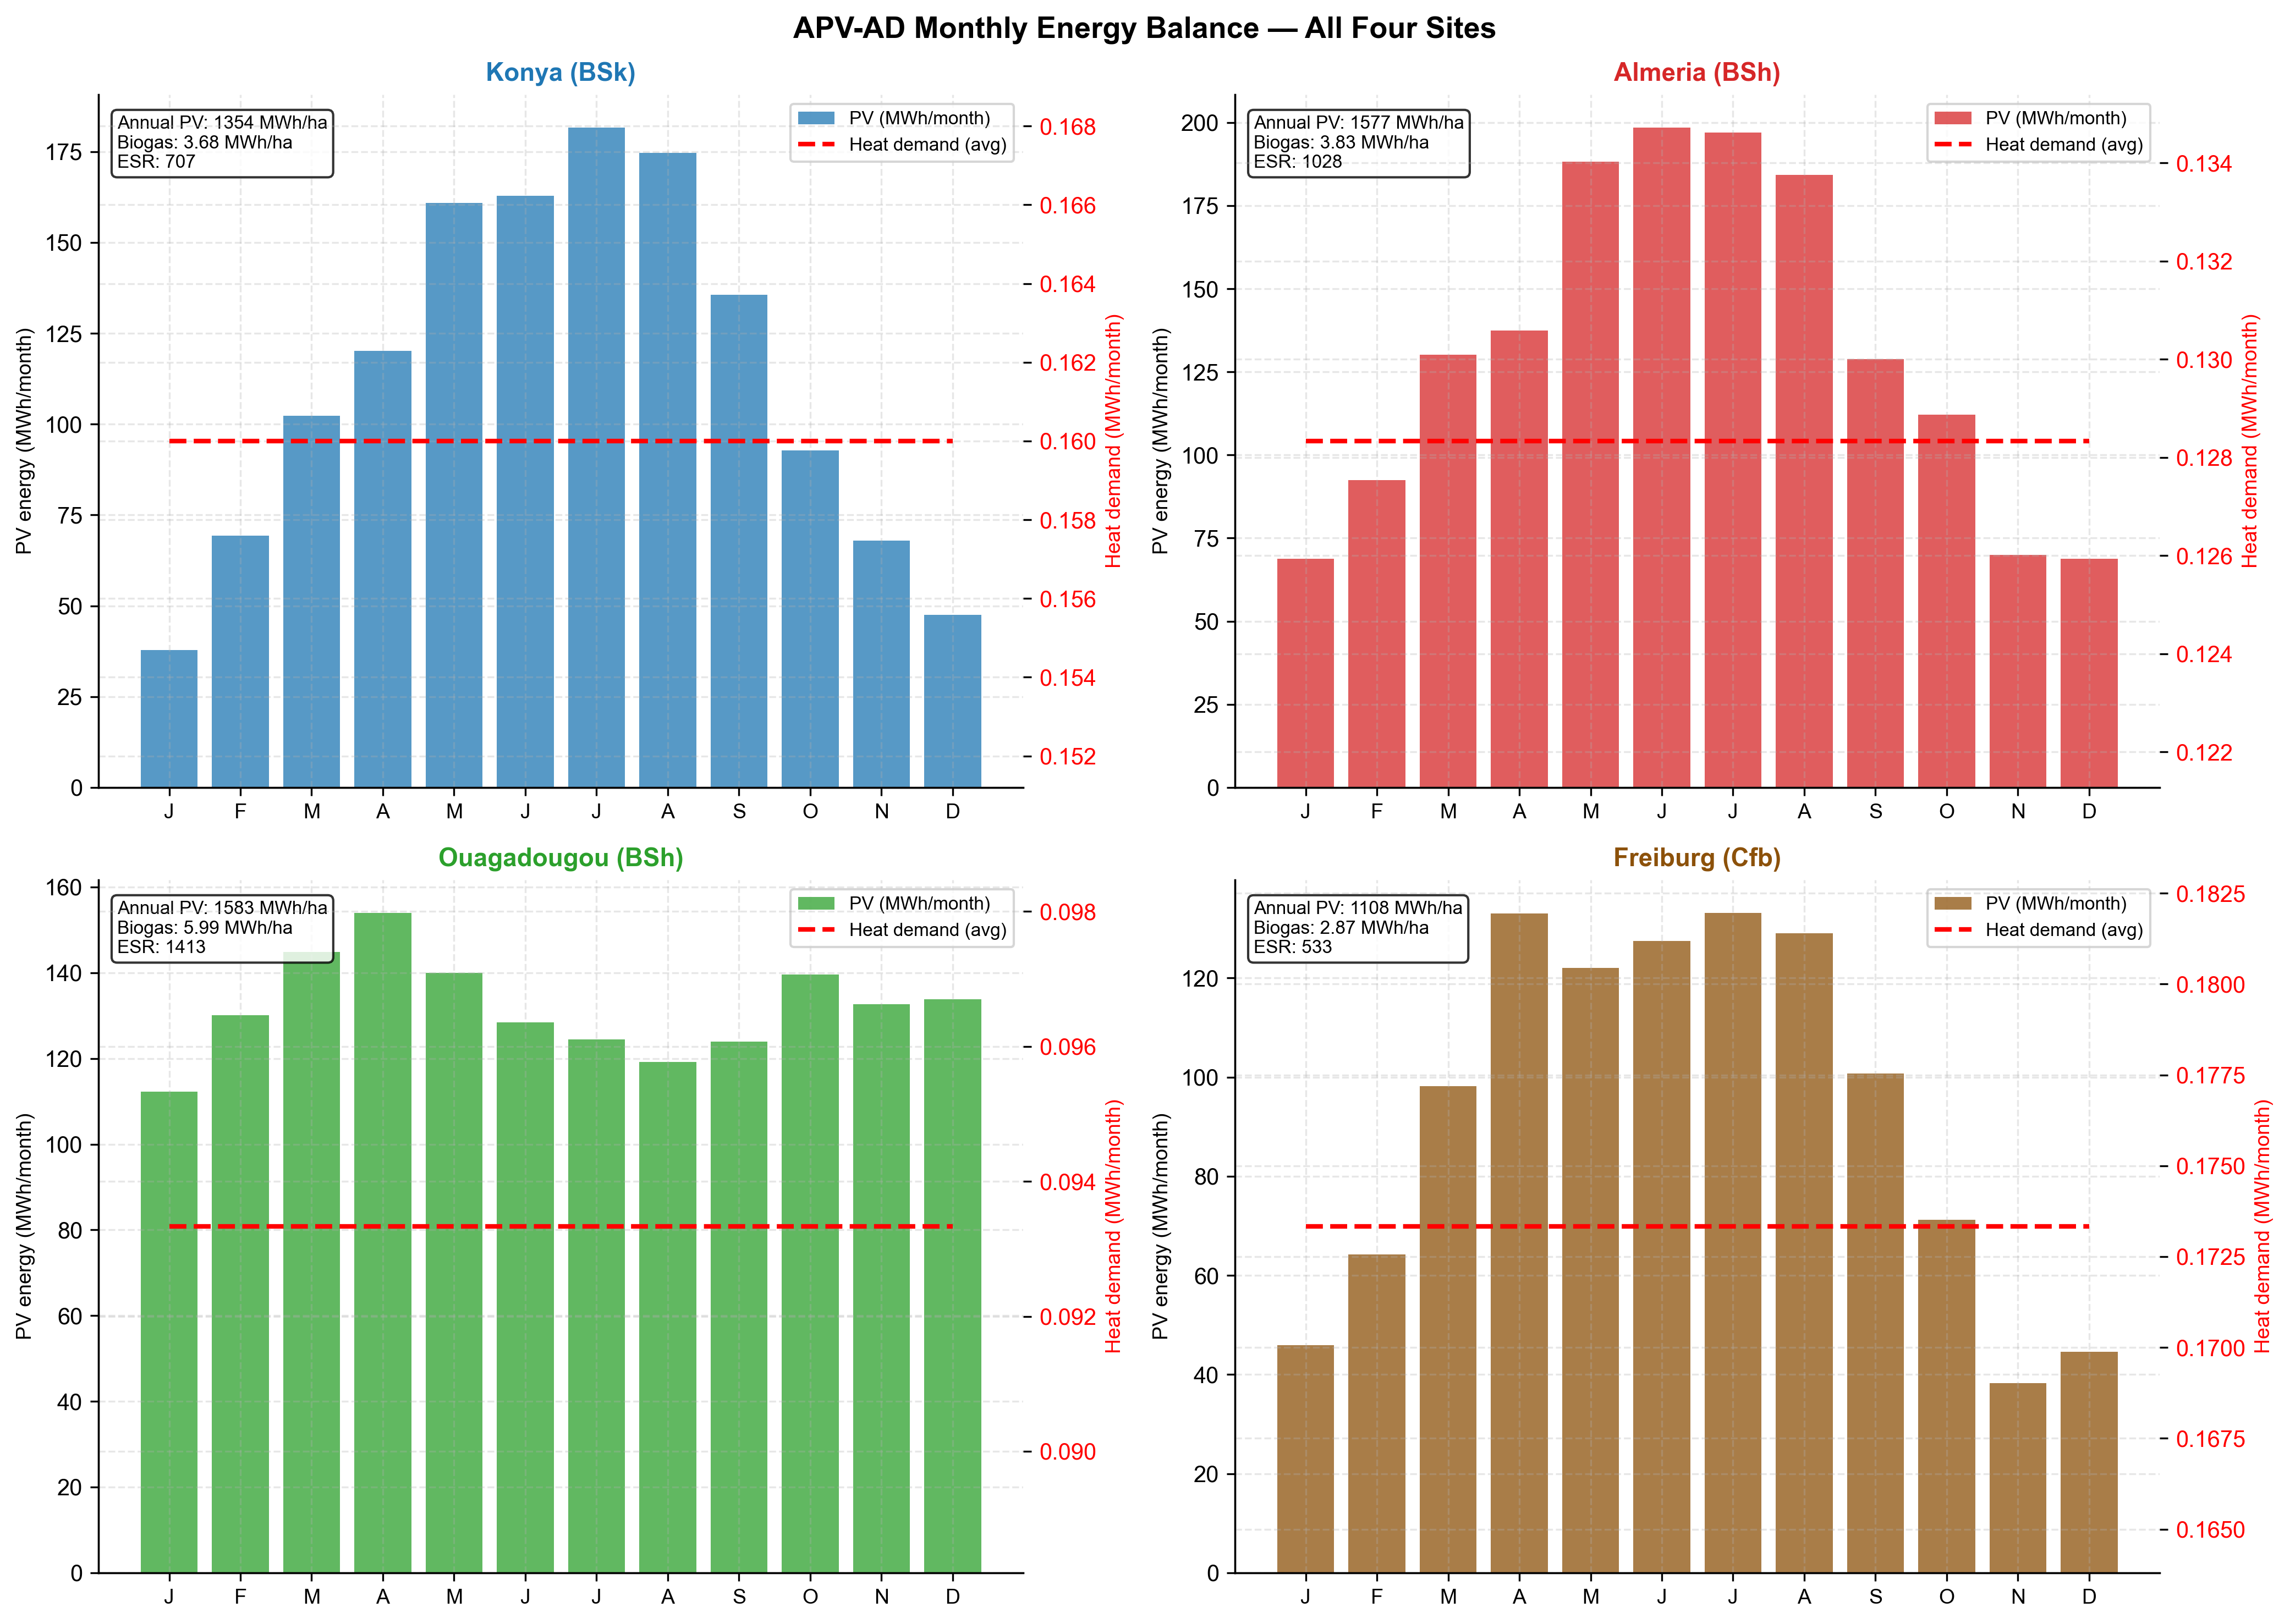
\includegraphics[width=\textwidth]{figures/fig04_energy_monthly.png}
	\caption{Monthly energy balance for all four sites. Bars: monthly PV
		generation (MWh\,month$^{-1}$). Dashed line: monthly average digester
		heat demand. The heat demand is nearly constant year-round at all
		sites because $T_{\text{dig,eff}}$ is clipped to
		$[26,\,37]\,^{\circ}$C (Equation~\ref{eq:tdig}), decoupling heat
		demand from the seasonal PV profile.}
	\label{fig:energy}
\end{figure}

Four observations characterize the energy performance across sites.

\textbf{PV generation follows the GHI gradient.} Annual PV output
ranges from 1\,108\,MWh\,ha$^{-1}$ (Freiburg) to
1\,583\,MWh\,ha$^{-1}$ (Ouagadougou), tracking the GHI gradient
as expected. The ratio of PV sold to PV total is 94--95\% at all
sites, reflecting the near-minimum $f_{\text{PV,heat}}^* \approx 0.05$
at the optimized design: only 5\% of PV output is allocated to
digester heating.

\textbf{Biogas production is dominated by temperature regime.}
Biogas output varies from 2.87\,MWh\,ha$^{-1}$ (Freiburg) to
5.99\,MWh\,ha$^{-1}$ (Ouagadougou), a factor of 2.1$\times$.
This variation is driven primarily by the annual average BMP, which
ranges from 140.4\,NmL\,CH$_4$\,gVS$^{-1}$ (Freiburg) to
234.0\,NmL\,CH$_4$\,gVS$^{-1}$ (Ouagadougou). At Ouagadougou,
the tropical ambient temperature (\SI{28.5}{\celsius} annual mean)
raises $T_{\text{dig,eff}}$ to 33.2\,\si{\celsius} year-round,
approaching the mesophilic optimum and maintaining BMP at
$\sim$300\,NmL\,CH$_4$\,gVS$^{-1}$ with minimal seasonal
variation. At Konya and Freiburg, winter ambient temperatures
below 0\,\si{\celsius} suppress $T_{\text{dig,eff}}$ to the
minimum threshold of 26\,\si{\celsius}, reducing BMP to
approximately 130--140\,NmL\,CH$_4$\,gVS$^{-1}$ during
December--February. The Arrhenius-corrected annual average BMP
of 148.8\,NmL\,CH$_4$\,gVS$^{-1}$ at Konya and
140.4\,NmL\,CH$_4$\,gVS$^{-1}$ at Freiburg represent a 50--53\%
suppression relative to the mesophilic reference, quantifying
the thermal penalty of cold climates on biogas yield.

\textbf{Thermal self-sufficiency is confirmed at all sites.}
ESR ranges from 533 (Freiburg) to 1\,413 (Ouagadougou), orders of
magnitude above the threshold of 1.0. Zero biogas is consumed for
digester heating at any site, even at Freiburg in January. This
confirms that the PV array provides far more energy than the
digester requires under the optimal $f_{\text{PV,heat}}^* = 0.05$
design: 5\% of 1\,108\,MWh\,ha$^{-1}$ = 55\,MWh is available
for heating against a total heat demand of only
2.08\,MWh\,ha$^{-1}$ at Freiburg. The implication is that
$LER_{\text{biogas}} < 1$ is driven entirely by the reduction in
crop residues under APV shading, not by any thermal penalty on
the digestion process.

\textbf{Heat demand is lowest at Ouagadougou.} Despite the largest
digester volume (3.52\,m$^3$), Ouagadougou has the lowest heat
demand (1.12\,MWh\,ha$^{-1}$\,yr$^{-1}$) because the small
temperature difference between ambient (\SI{28.5}{\celsius} mean)
and digester (\SI{33.2}{\celsius} effective) minimises both
conductive wall losses ($Q_{\text{loss}}$) and substrate heating
demand ($Q_{\text{inflow}}$). Freiburg has the highest heat demand
(2.08\,MWh\,ha$^{-1}$\,yr$^{-1}$) despite having the smallest
digester (3.10\,m$^3$), driven by the large
$\overline{T}_{\text{dig}} - \overline{T}_{\text{amb}}$ differential
of approximately 14.6\,K in winter months.

% ---------------------------------------------------------------------------
\subsection{Climate Gradient and Non-Monotone eLER Ordering}
\label{sec:results_gradient}
% ---------------------------------------------------------------------------

\hspace{1cm}Figure~\ref{fig:gradient} presents the four-site climate
gradient alongside the corresponding eLER and $LER_{\text{2C}}$ values.
The central finding of this study emerges from this comparison: the eLER
ordering does not follow the solar resource gradient.

\begin{figure}[H]
	\centering
	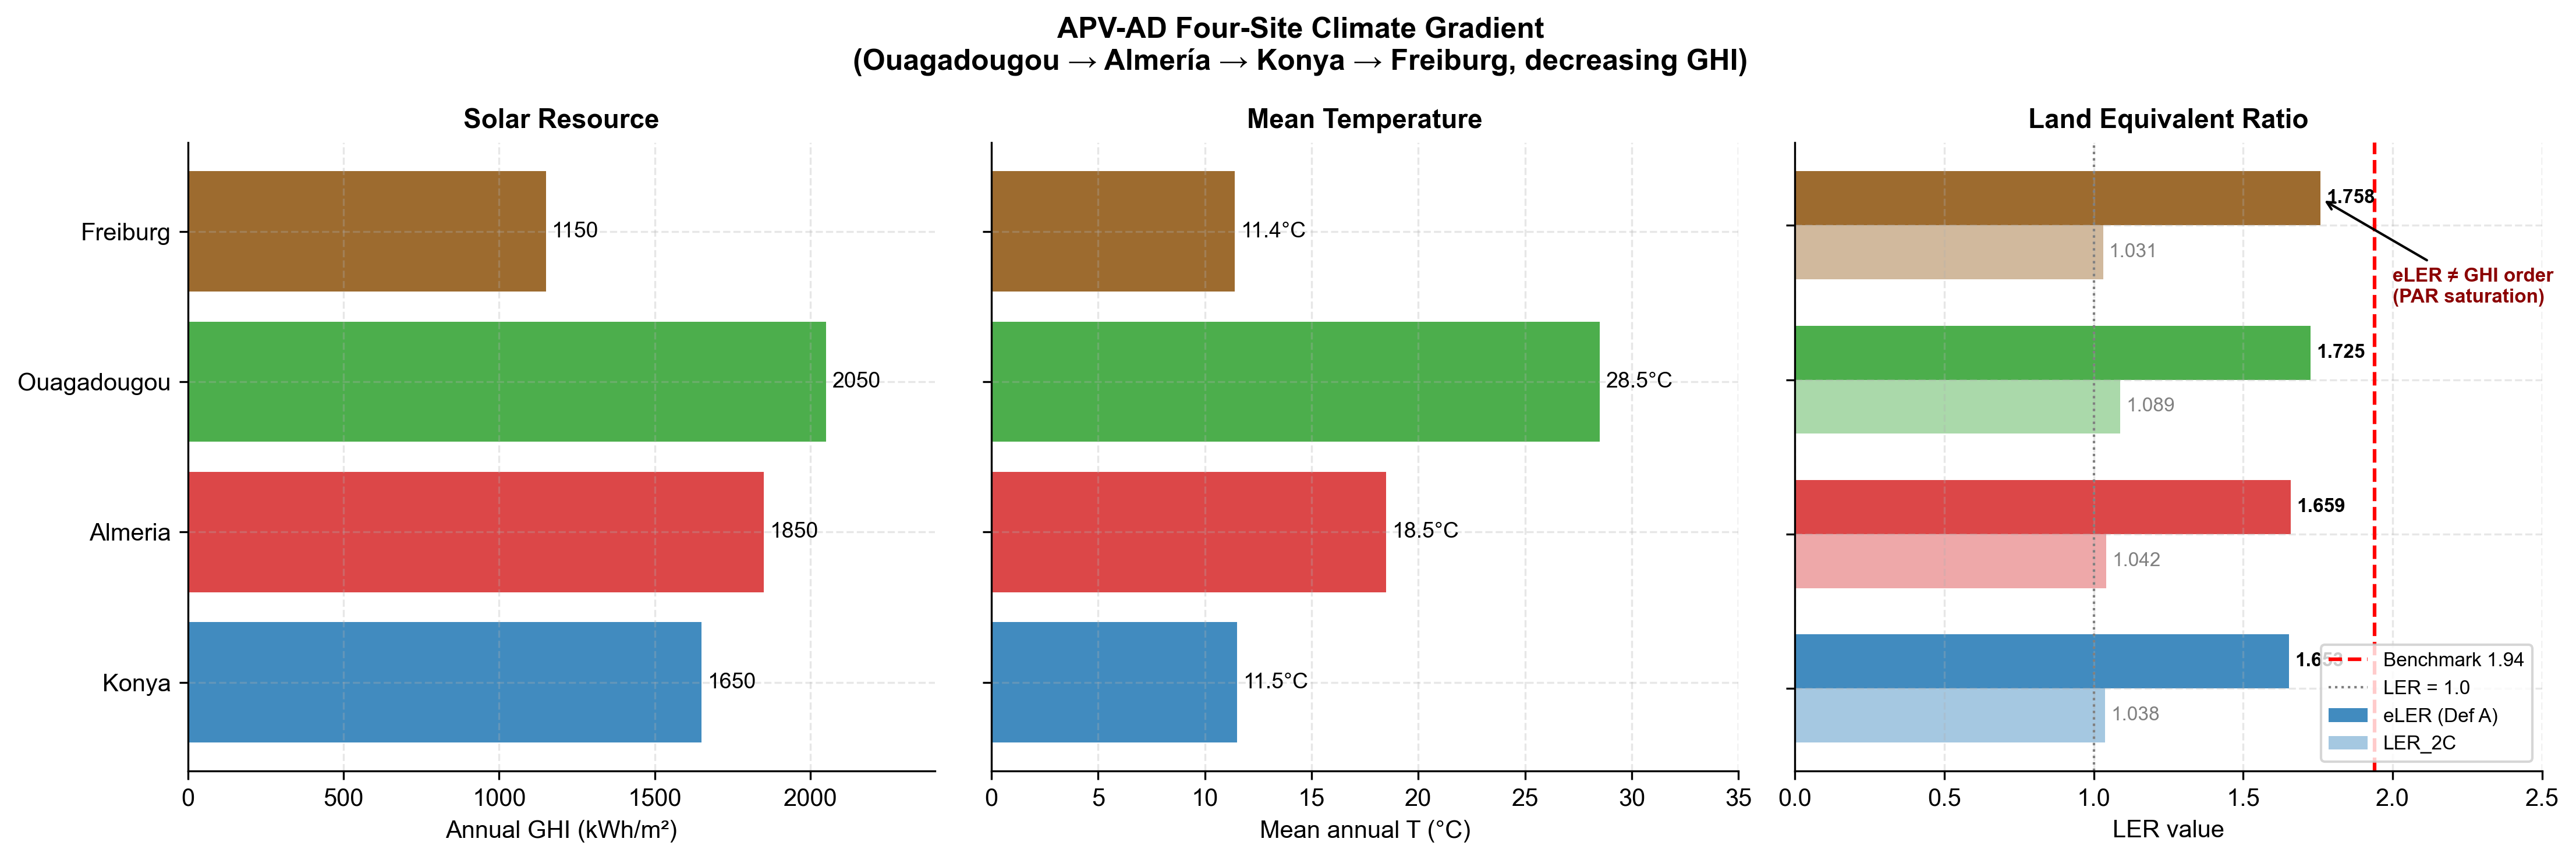
\includegraphics[width=\textwidth]{figures/fig05_climate_gradient.png}
	\caption{Four-site climate gradient. Left panel: annual GHI
		(kWh\,m$^{-2}$). Centre panel: mean annual air temperature
		(\si{\celsius}). Right panel: eLER (Definition~A, solid bars) and
		$LER_{\text{2C}}$ (faded bars) with the red dashed line at the
		published benchmark of 1.94~\citep{riaz2022}. The annotation
		highlights the non-monotone result: Freiburg (lowest GHI) achieves
		the highest eLER.}
	\label{fig:gradient}
\end{figure}

The solar resource and eLER rankings are:
\begin{align*}
	\text{GHI:} \quad
	&\text{Ouagadougou} (2050) > \text{Almer\'{i}a} (1850)
	> \text{Konya} (1650) > \text{Freiburg} (1150) \\
	\text{eLER:} \quad
	&\text{Freiburg} (1.758) > \text{Ouagadougou} (1.725)
	> \text{Almer\'{i}a} (1.659) > \text{Konya} (1.653)
\end{align*}

The eLER ordering is the inverse of the GHI ordering at the two
extremes: Freiburg, with the lowest annual irradiance
(1\,150\,kWh\,m$^{-2}$), achieves the highest eLER (1.758), while
Konya, with 43\% more irradiance (1\,650\,kWh\,m$^{-2}$), achieves
the lowest eLER (1.653).

\textbf{Mechanism: PAR saturation inflates the LER$_{\text{crop}}$
	denominator at high-irradiance sites.}
The PAR integral formulation (Equation~\ref{eq:lercrop}) clips the
numerator at $PAR_{\text{sat}} = \SI{174}{W\,m^{-2}}$ but leaves the
denominator uncapped. At high-irradiance sites, mean daytime
$PAR_{\text{open}}$ frequently exceeds $PAR_{\text{sat}}$, making the
denominator large while the numerator is bounded. The following
site-specific analysis quantifies this effect.

At Konya, mean growing-season daytime GHI exceeds
$PAR_{\text{sat}} / f_{\text{PAR}} = 174 / 0.48 =
\SI{362}{W\,m^{-2}}$ for approximately 60\% of daylight hours,
meaning the open-field denominator accumulates uncapped PAR for more
than half the season while the APV numerator is clipped at
$PAR_{\text{sat}}$ for the same hours. The result is
$LER_{\text{crop}} = 0.363$ despite the high solar resource.

At Freiburg, mean growing-season daytime GHI exceeds
\SI{362}{W\,m^{-2}} for only approximately 20\% of daylight hours.
The denominator accumulates proportionally less uncapped PAR,
making the ratio $\int\min(PAR_{\text{AV}}, PAR_{\text{sat}})\,dt /
\int PAR_{\text{open}}\,dt$ more favourable. The result is
$LER_{\text{crop}} = 0.371$, marginally higher than Konya despite
Freiburg receiving 500\,kWh\,m$^{-2}$ less annual irradiance.

Since $LER_{\text{PV}}$ (Definition~A) is near-uniform across sites
(0.660--0.691, as established in Section~\ref{sec:results_eler}),
and $LER_{\text{biogas}}$ is highest at Freiburg (0.727) due to the
lower open-field reference yield, the combination of a slightly
higher $LER_{\text{crop}}$ and the highest $LER_{\text{biogas}}$
gives Freiburg the overall eLER advantage.

\textbf{Design implication.} For tomato cultivation
($PAR_{\text{sat}} = \SI{174}{W\,m^{-2}}$), integrated APV--AD
systems deliver proportionally higher land-use efficiency in
moderate-irradiance temperate climates than in high-irradiance
semi-arid climates. This result is crop-specific: shade-tolerant
crops with lower $PAR_{\text{sat}}$ (e.g.\ lettuce,
\SI{76}{W\,m^{-2}}) would be saturated more frequently at all
sites, potentially eliminating or reversing the gradient. Multi-crop
generalization is identified as a priority for future work
(Section~\ref{sec:discussion}).
% ---------------------------------------------------------------------------
\subsection{4E Analysis: Energetic, Economic, Energo-Economic,
	and Environmental Performance}
\label{sec:results_4e}
% ---------------------------------------------------------------------------

\hspace{1cm}Figure~\ref{fig:4e} presents the 4E dashboard for all
four sites under Scenario S0. Table~\ref{tab:capex} reports the CAPEX
breakdown; Table~\ref{tab:economics} summarises the key investment
metrics for Scenarios S0 and S6 across all sites.

\begin{figure}[H]
	\centering
	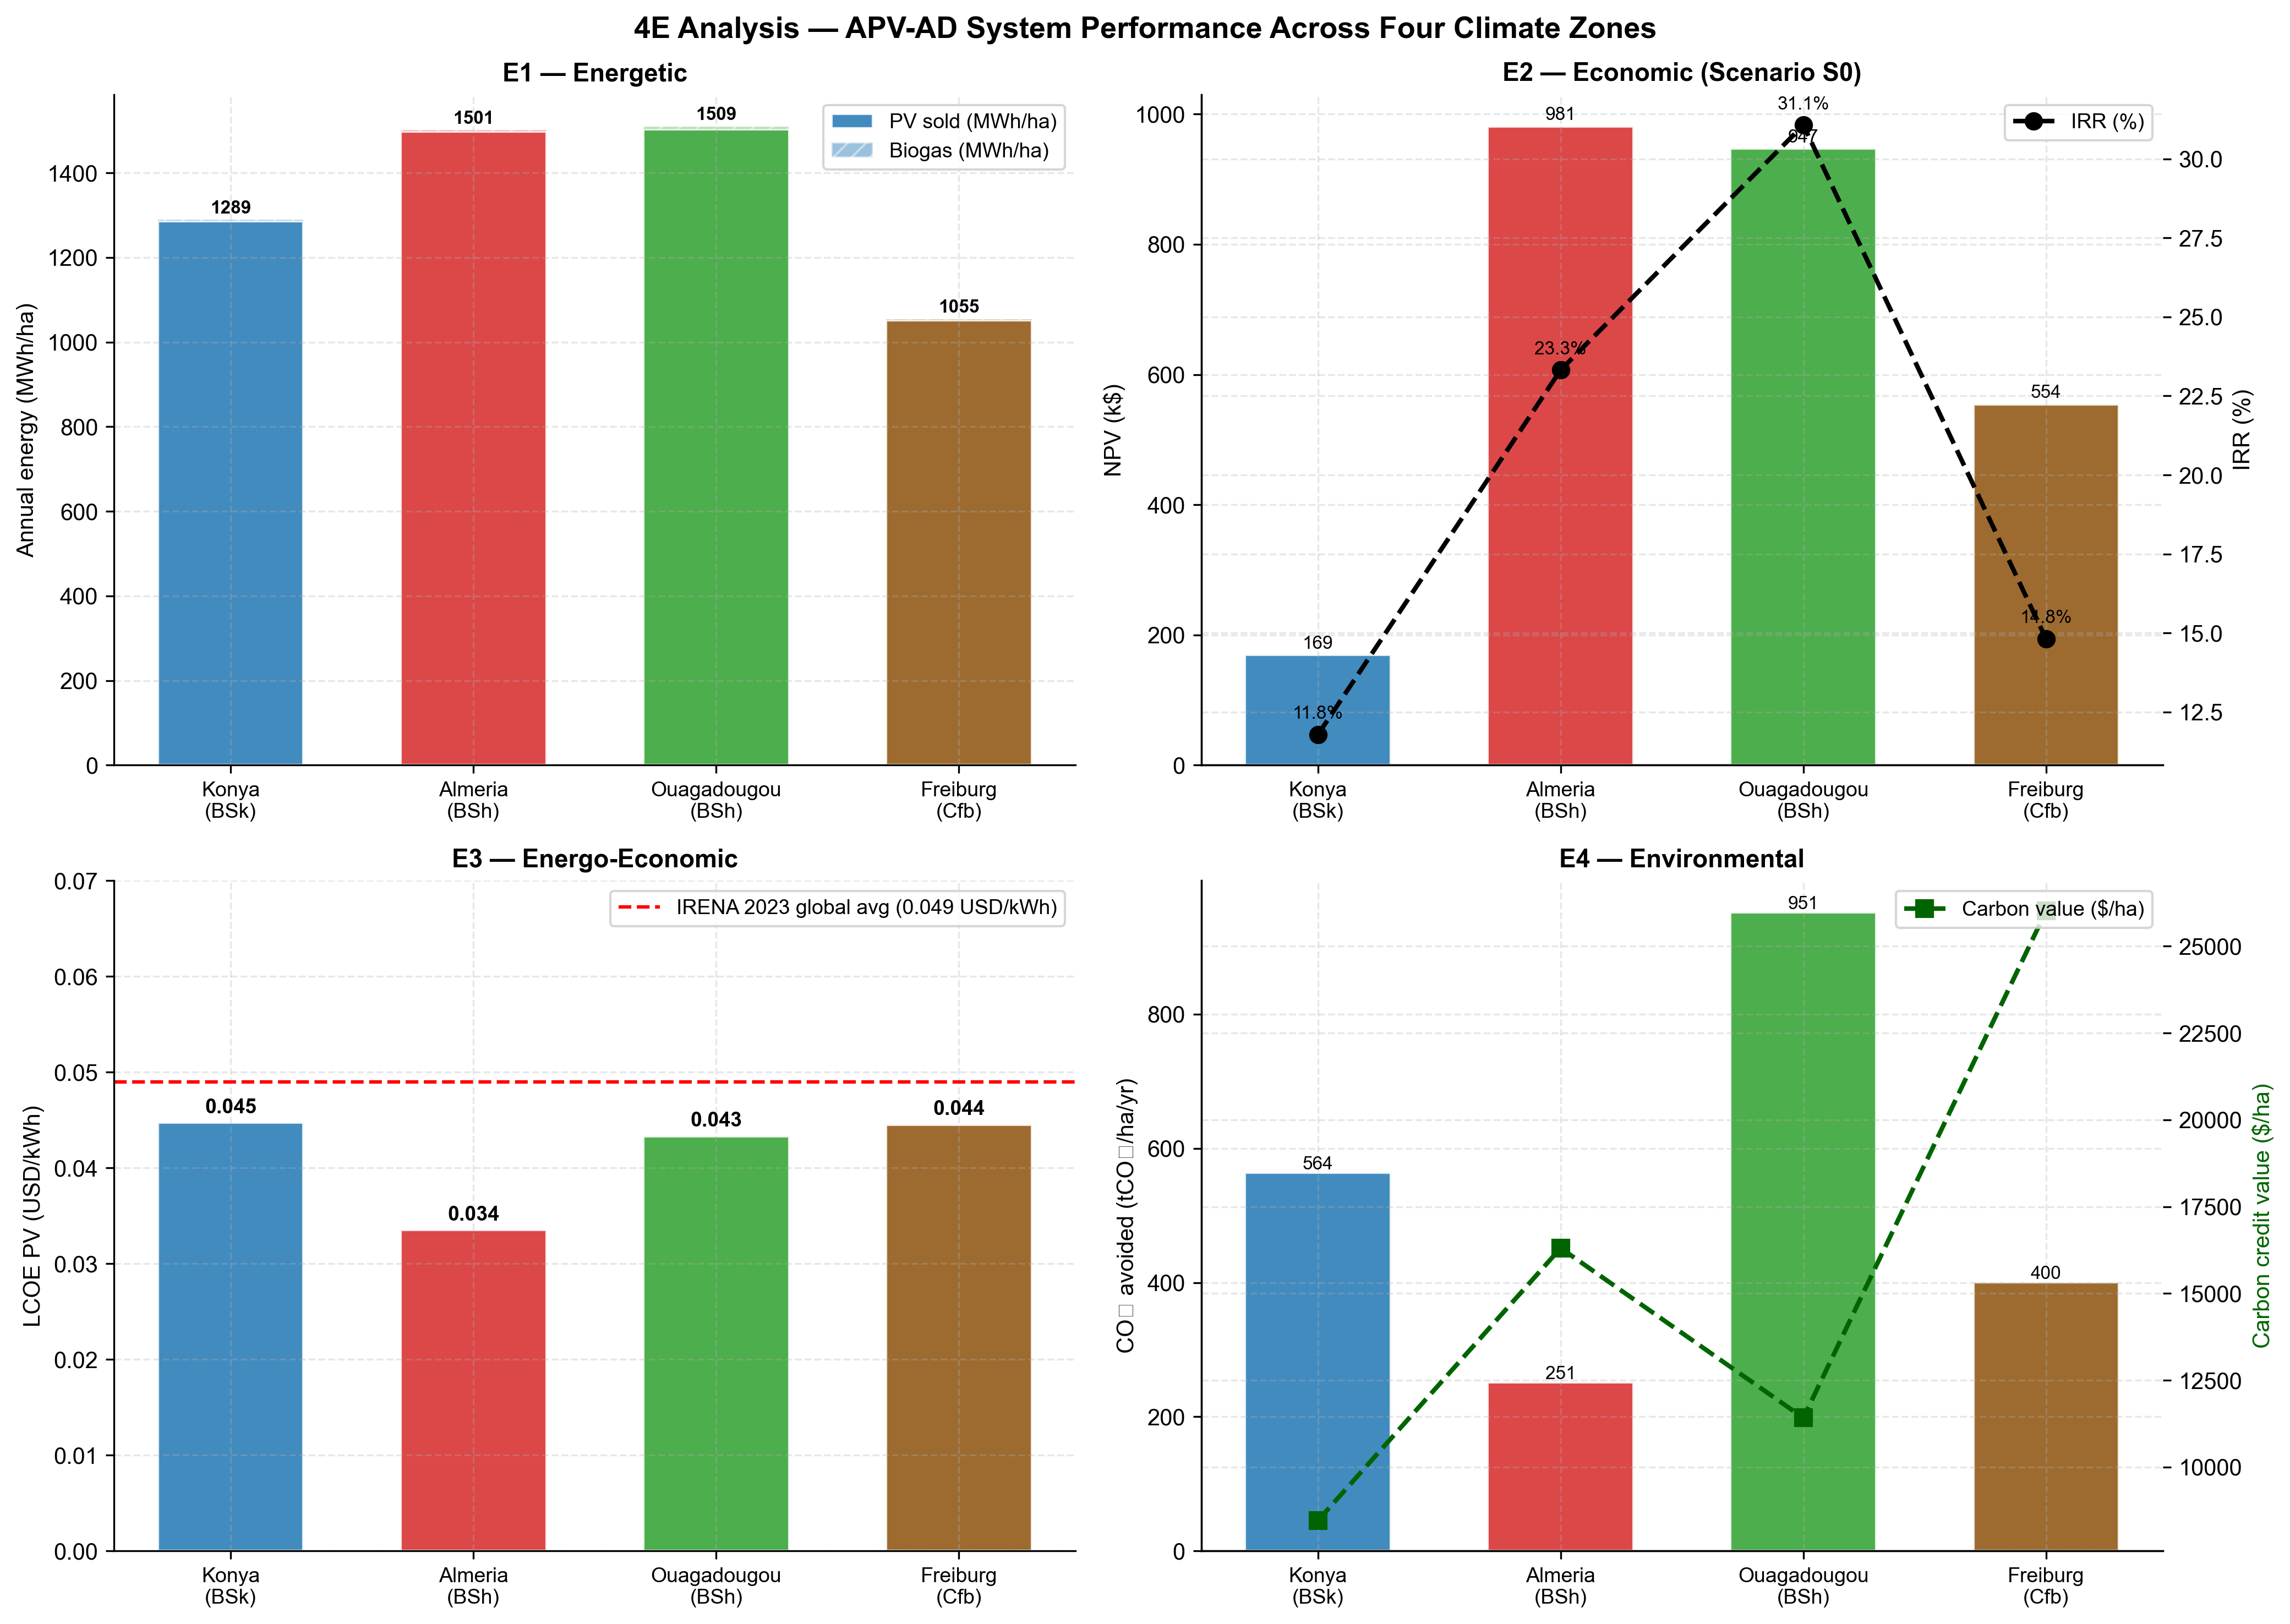
\includegraphics[width=\textwidth]{figures/fig06_4E_dashboard.png}
	\caption{4E performance dashboard for all four sites (Scenario S0).
		Top left (E1): annual PV and biogas energy (MWh\,ha$^{-1}$).
		Top right (E2): NPV (k\$, bars) and IRR (\%, line).
		Bottom left (E3): LCOE$_{\text{PV}}$ (USD\,kWh$^{-1}$) with the
		IRENA 2023 global benchmark (red dashed line).
		Bottom right (E4): CO$_2$ avoided (tCO$_2$\,ha$^{-1}$\,yr$^{-1}$,
		bars) and carbon credit value (USD\,ha$^{-1}$, line).}
	\label{fig:4e}
\end{figure}

\subsubsection{CAPEX Breakdown}

\begin{table}[H]
	\caption{CAPEX breakdown for all four sites (1\,ha, Scenario S0).
		PV CAPEX based on 1\,419 modules $\times$ 550\,W$_p$ $\times$
		\$0.63\,W$_p^{-1}$. AD CAPEX based on optimal $V_{\text{dig}}^*$
		$\times$ \$800\,m$^{-3}$.}
	\label{tab:capex}
	\centering
	\begin{tabular}{lcccc}
		\toprule
		\textbf{Component} & \textbf{Konya} & \textbf{Almer\'{i}a}
		& \textbf{Ouagadougou} & \textbf{Freiburg} \\
		\midrule
		PV array (k\$)              & 493 & 493 & 493 & 493 \\
		AD digester (k\$)           & 3   & 3   & 3   & 2   \\
		Agricultural infra. (k\$)   & 3   & 3   & 3   & 3   \\
		Balance of plant (k\$)      & 74  & 74  & 74  & 74  \\
		\textbf{Total CAPEX (k\$)}  & \textbf{573} & \textbf{573}
		& \textbf{573} & \textbf{572} \\
		Annual O\&M (k\$\,yr$^{-1}$) & 8.6 & 8.6 & 8.6 & 8.6 \\
		\bottomrule
	\end{tabular}
\end{table}

Total CAPEX is near-identical across sites (\$572--573\,k\,ha$^{-1}$)
because the number of modules (1\,419) and the module unit cost
dominate the budget: PV accounts for 86\% of total CAPEX. The AD
digester contributes only 0.3--0.5\% of CAPEX, reflecting the
small optimal digester volumes (3.10--4.14\,m$^3$). The marginal
cost of adding an AD unit to an existing APV system is therefore
negligible relative to the PV investment, making the biogas revenue
stream a low-risk addition.

\subsubsection{Investment Metrics (E2)}

\begin{table}[H]
	\caption{Investment metrics for Scenarios S0 (baseline) and S6
		(carbon credit) at all four sites. NPV computed at site-specific
		discount rates over 20-year project life. IRR solved by bisection.
		LCOE$_{\text{PV}}$ uses PV CAPEX and annual PV sold.}
	\label{tab:economics}
	\centering
	\begin{tabular}{llcccc}
		\toprule
		\textbf{Scenario} & \textbf{Metric} & \textbf{Konya}
		& \textbf{Almer\'{i}a} & \textbf{Ouagadougou} & \textbf{Freiburg} \\
		\midrule
		\multirow{5}{*}{S0}
		& Gross revenue (k\$\,yr$^{-1}$) & 110 & 211 & 278 & 166 \\
		& Net CF (k\$\,yr$^{-1}$)        & 101 & 202 & 269 & 157 \\
		& NPV (k\$)                       & 169 & 981 & 947 & 554 \\
		& IRR (\%)                        & 11.8 & 23.3 & 31.1 & 14.8 \\
		& Payback (yr)                    & 7.6  & 4.2  & 3.2  & 6.3  \\
		\midrule
		\multirow{4}{*}{S6}
		& Net CF (k\$\,yr$^{-1}$)        & 113 & 234 & 283 & 218 \\
		& NPV (k\$)                       & 252 & 1\,168 & 1\,044 & 878 \\
		& IRR (\%)                        & 13.5 & 26.3 & 33.1 & 19.8 \\
		& Payback (yr)                    & 6.8  & 3.8  & 3.0  & 4.9  \\
		\bottomrule
	\end{tabular}
\end{table}

Four economic findings are noteworthy.

\textbf{Ouagadougou offers the strongest investment case.}
Under S0, Ouagadougou achieves IRR = 31.1\% and payback = 3.2\,yr,
driven by the combination of the highest electricity price
(\$0.12\,kWh$^{-1}$), the highest PV output (1\,583\,MWh\,ha$^{-1}$),
and the highest biogas yield (5.99\,MWh\,ha$^{-1}$). The IRR exceeds
the site discount rate (10\%) by 21.1 percentage points, providing
a large investment margin.

\textbf{Konya is marginal but viable under S0.}
IRR = 11.8\% exceeds the 8\% discount rate by only 3.8 percentage
points, and NPV = 169\,k\$ is the lowest of the four sites. The
primary constraint is the low electricity tariff
(\$0.06\,kWh$^{-1}$), which limits PV revenue despite the
competitive PV output (1\,354\,MWh\,ha$^{-1}$).

\textbf{S6 (carbon credit) is the dominant economic scenario
	at all sites.} S6 raises IRR by 1.7--5.0 percentage points above
S0, with the largest absolute improvement at Freiburg
(+5.0\,pp, from 14.8\% to 19.8\%) driven by the high EU ETS
carbon price (\$65\,tCO$_2^{-1}$) and the large CO$_2$ avoidance
from displacing Germany's carbon-intensive grid
(EF = 0.380\,tCO$_2$\,MWh$^{-1}$). Figure~\ref{fig:scenarios}
shows the full scenario comparison.

\textbf{LCOE$_{\text{PV}}$ is competitive at all sites.}
As shown in the E3 panel of Figure~\ref{fig:4e}, LCOE$_{\text{PV}}$
ranges from \$0.034\,kWh$^{-1}$ (Almer\'{i}a) to
\$0.045\,kWh$^{-1}$ (Konya). Almer\'{i}a approaches the IRENA 2023
global utility-scale solar benchmark of \$0.049\,kWh$^{-1}$, while
the other three sites remain within 9--19\% above it --- a premium
attributable to the elevated APV mounting structure, which carries a
40\% CAPEX premium over standard ground-mount.

\begin{figure}[H]
	\centering
	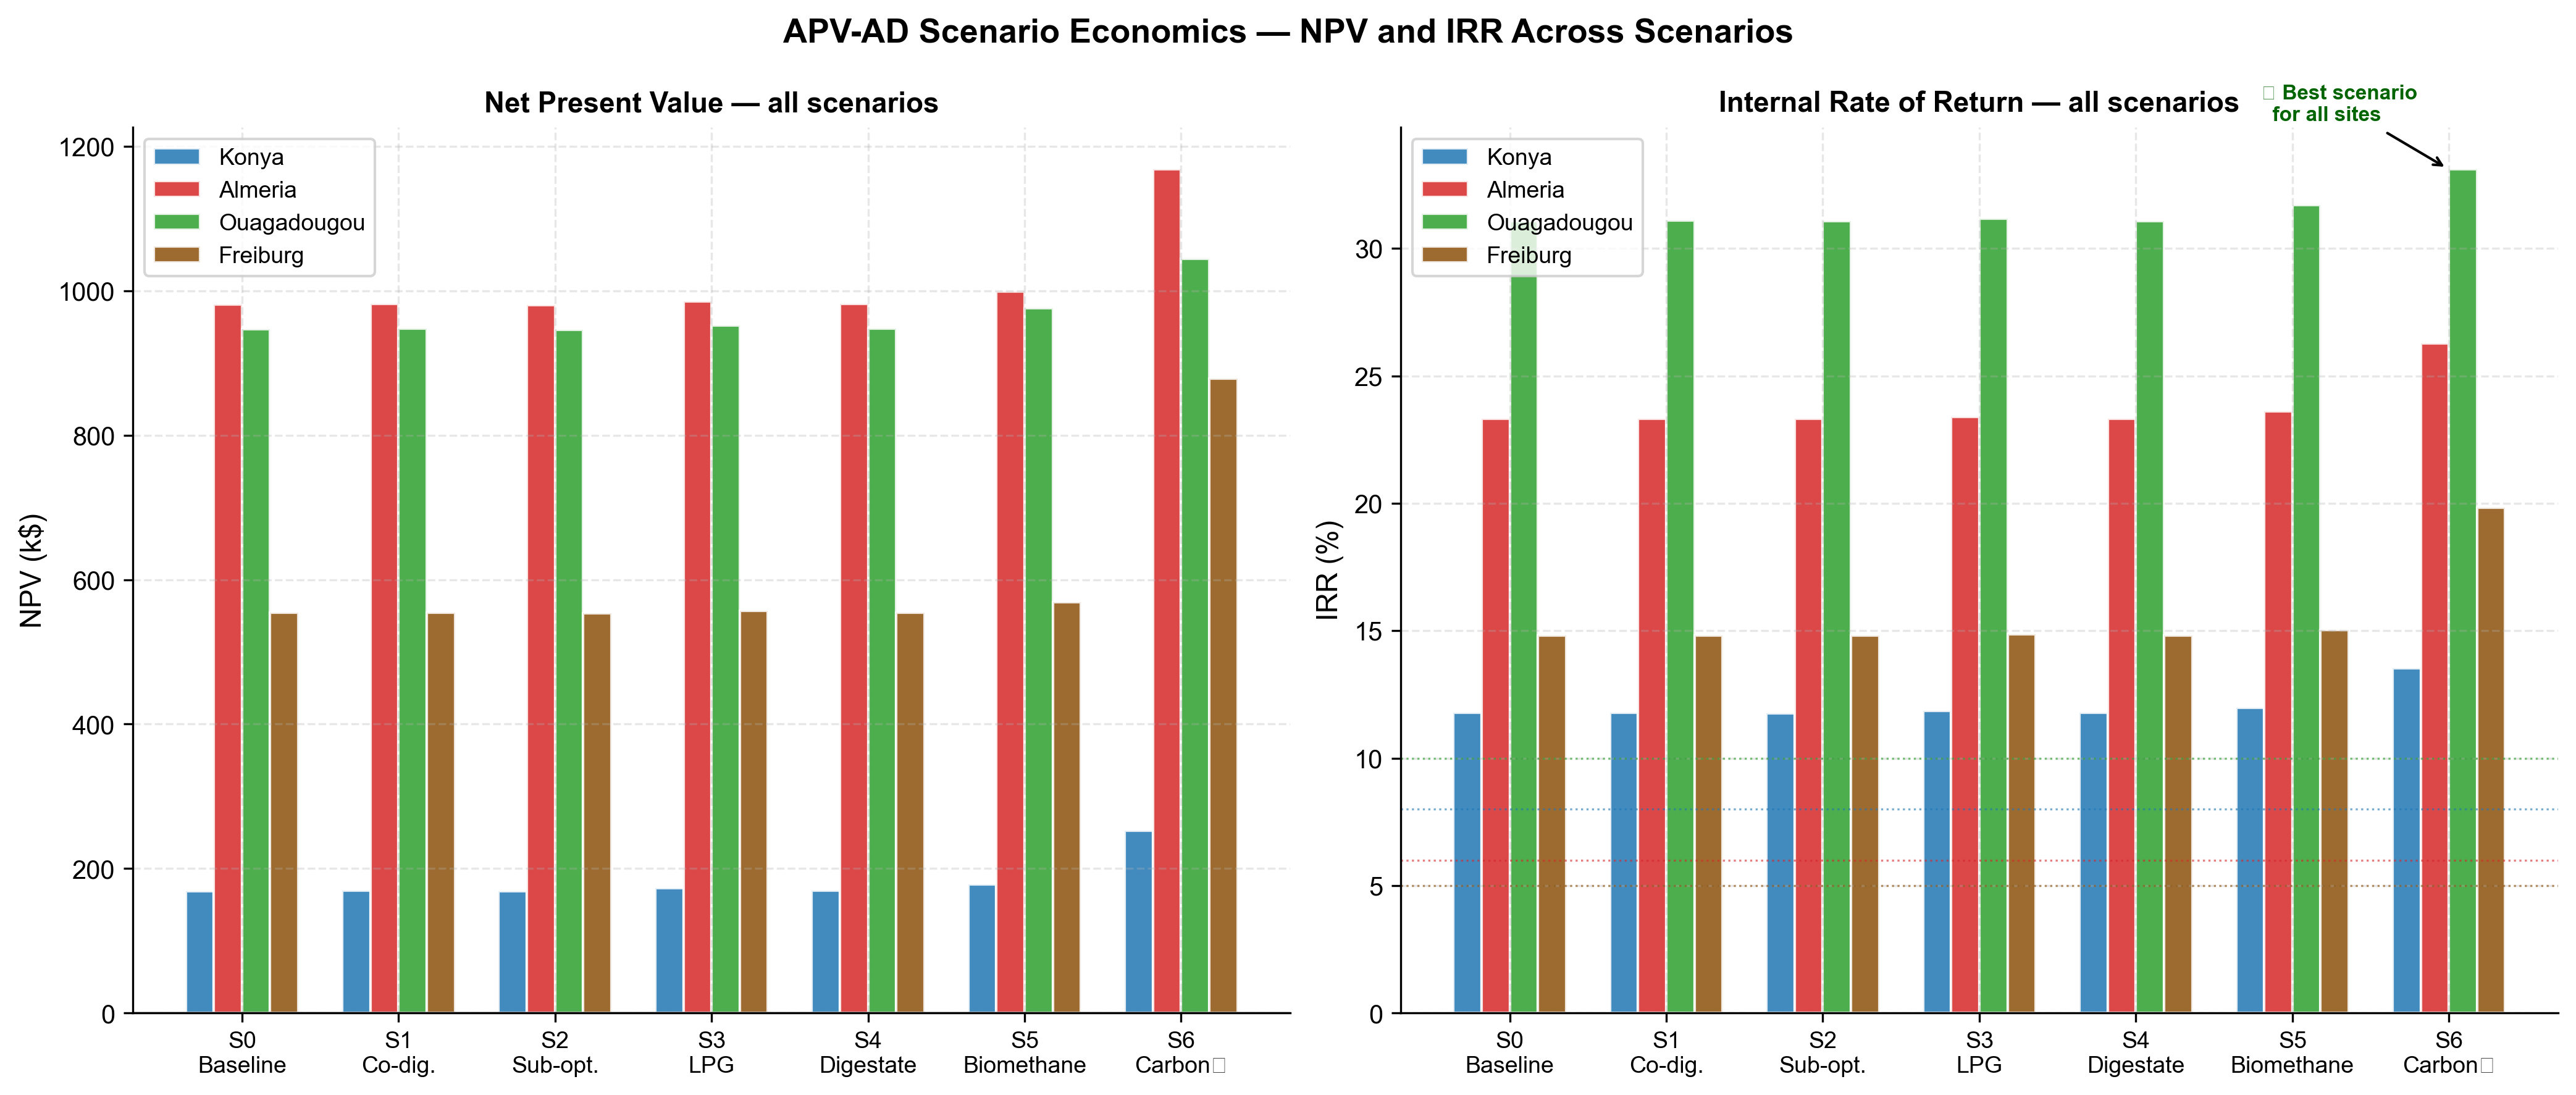
\includegraphics[width=\textwidth]{figures/fig07_scenarios.png}
	\caption{Scenario economics for all four sites. Left panel: NPV (k\$)
		for Scenarios S0--S6. Right panel: IRR (\%) for Scenarios S0--S6,
		with dotted horizontal lines indicating site-specific discount rates.
		S6 (carbon credit, starred) is the dominant scenario at all sites.}
	\label{fig:scenarios}
\end{figure}

\subsubsection{Environmental Performance (E4)}

\hspace{1cm}Annual CO$_2$ avoidance ranges from
251\,tCO$_2$\,ha$^{-1}$ (Almer\'{i}a) to
951\,tCO$_2$\,ha$^{-1}$ (Ouagadougou), driven primarily by the
grid emission factor of the displacement context. Ouagadougou's
diesel-dominated grid (EF = 0.632\,tCO$_2$\,MWh$^{-1}$) combined
with the highest PV output (1\,503\,MWh\,ha$^{-1}$ sold) produces
the largest absolute avoidance. Almer\'{i}a's already low-carbon
Spanish grid (EF = 0.167\,tCO$_2$\,MWh$^{-1}$) limits avoidance
despite competitive PV output. The carbon credit value --- the
monetary expression of CO$_2$ avoidance under site-specific carbon
prices --- is highest at Freiburg (\$26\,015\,ha$^{-1}$\,yr$^{-1}$),
where the EU ETS price (\$65\,tCO$_2^{-1}$) amplifies the moderate
CO$_2$ avoidance (400\,tCO$_2$\,ha$^{-1}$) into the largest
financial environmental benefit of the four sites. This explains
why S6 provides the largest absolute NPV improvement at Freiburg
(+\$324\,k vs.\ S0).

% ---------------------------------------------------------------------------
\subsection{Water Savings and LER\textsubscript{water}}
\label{sec:results_water}
% ---------------------------------------------------------------------------

\hspace{1cm}Table~\ref{tab:water} reports growing-season water savings
and the corrected $LER_{\text{water}}$ for all four sites.
Figure~\ref{fig:water} compares the corrected growing-season metric
against the erroneous annual-denominator value used in prior studies.

\begin{table}[H]
	\caption{Growing-season water savings and $LER_{\text{water}}$
		for all four sites at the optimised design. The annual-denominator
		value is reported for literature comparison only and should not
		be used as an agronomic indicator.}
	\label{tab:water}
	\centering
	\begin{tabular}{lcccc}
		\toprule
		\textbf{Parameter} & \textbf{Konya} & \textbf{Almer\'{i}a}
		& \textbf{Ouagadougou} & \textbf{Freiburg} \\
		\midrule
		$W_{\text{saved}}$ (mm\,season$^{-1}$)   & 383  & 186  & 152  & 186  \\
		ET$_0$ season (mm)                         & 650  & 480  & 620  & 350  \\
		ET$_0$ annual (mm)                         & 2\,371 & 2\,463 & 3\,800 & 1\,160 \\
		\textbf{$LER_{\text{water}}$ season (\%)} & \textbf{20.6} & \textbf{18.6}
		& \textbf{15.5} & \textbf{22.8} \\
		$LER_{\text{water}}$ annual (\%) [ref.]   & 16.1 & 7.5  & 4.0  & 16.1 \\
		Correction factor                          & 1.3$\times$ & 2.5$\times$
		& 3.9$\times$ & 1.4$\times$ \\
		\bottomrule
	\end{tabular}
\end{table}

\begin{figure}[H]
	\centering
	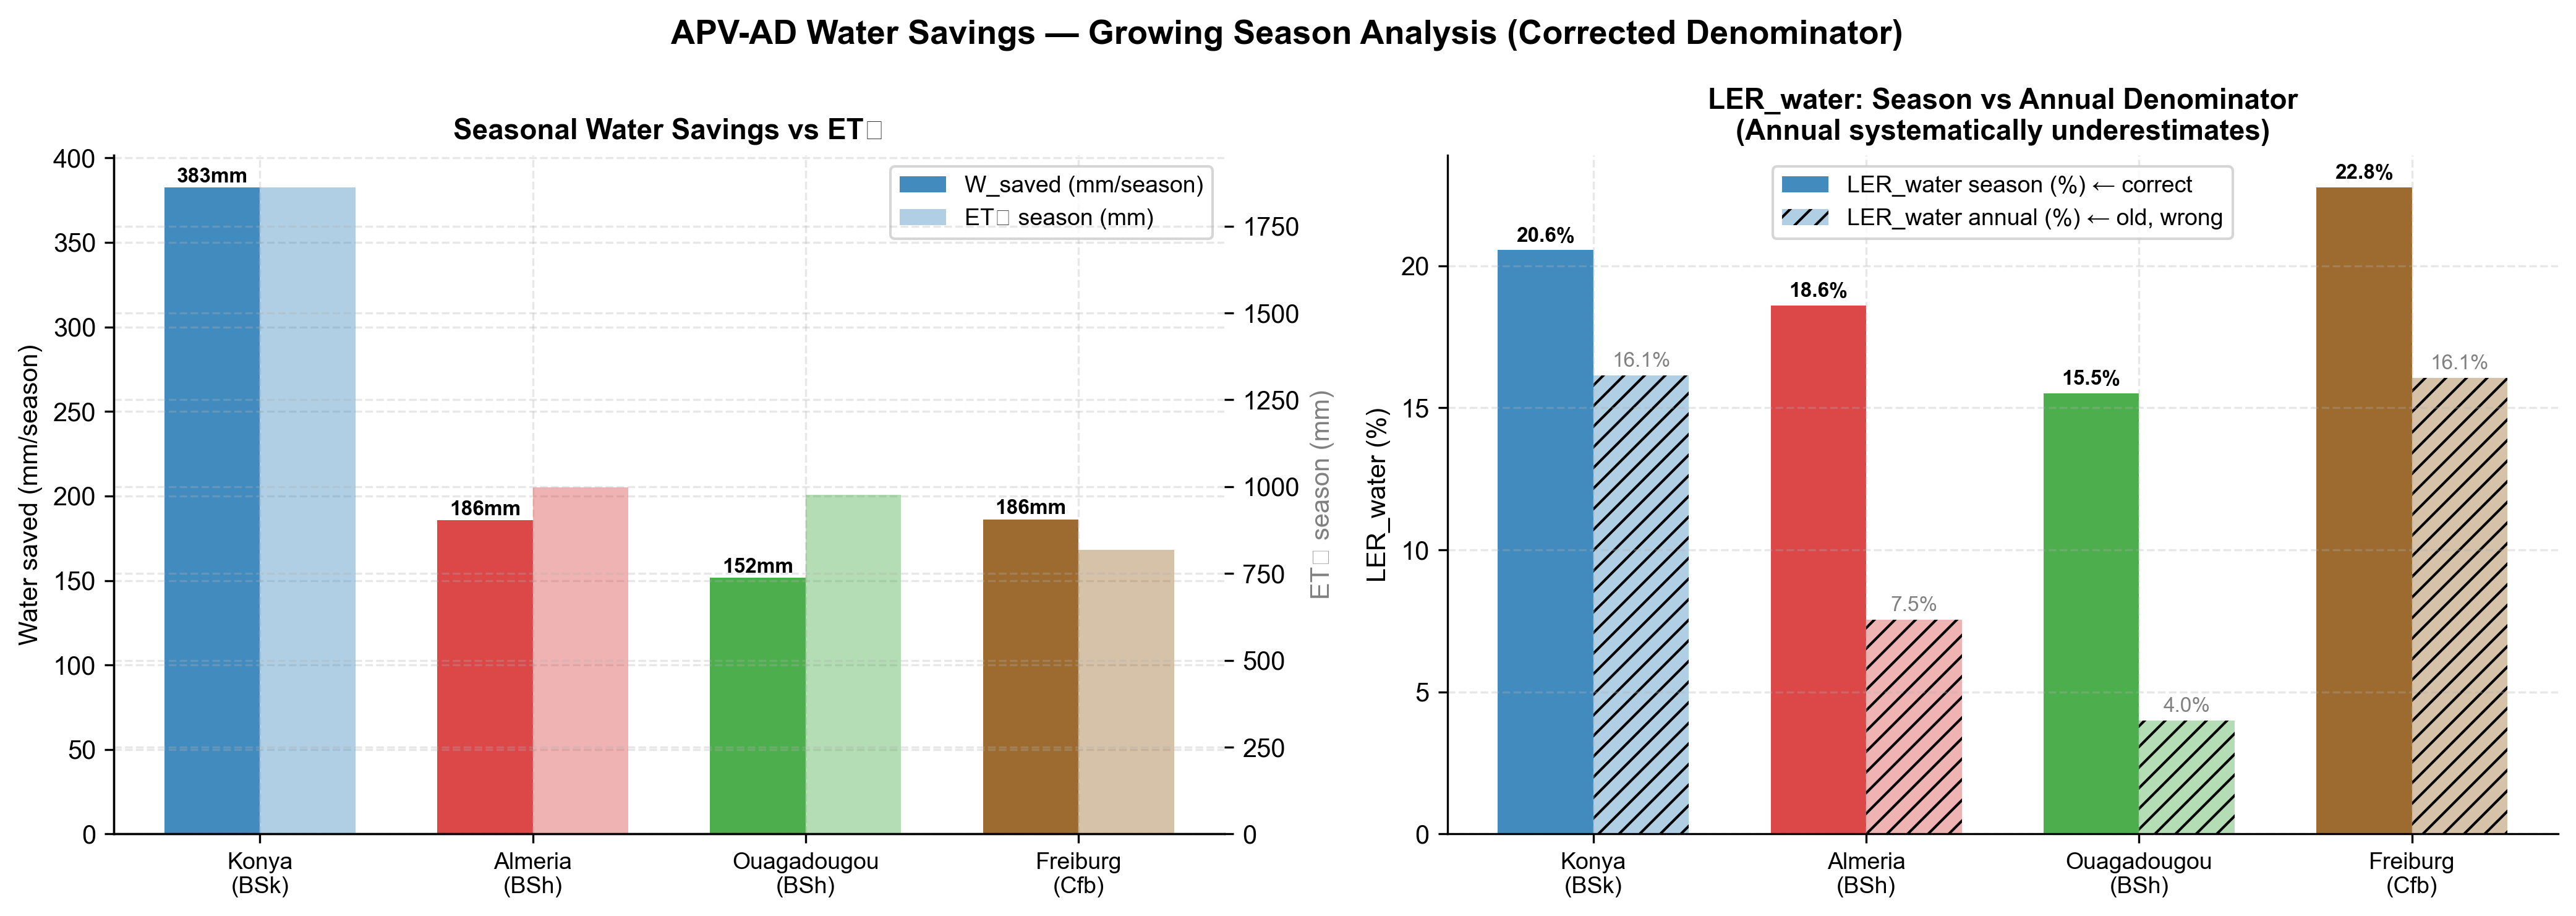
\includegraphics[width=\textwidth]{figures/fig08_water.png}
	\caption{Water savings analysis for all four sites. Left panel:
		absolute growing-season water savings $W_{\text{saved}}$
		(mm\,season$^{-1}$, bars) against seasonal ET$_0$ (mm, secondary
		bars). Right panel: $LER_{\text{water}}$ computed with the corrected
		growing-season denominator (solid bars) versus the erroneous
		annual-denominator value (hatched bars). The correction factor
		ranges from 1.3$\times$ (Konya) to 3.9$\times$ (Ouagadougou).}
	\label{fig:water}
\end{figure}

\textbf{Absolute water savings are largest at Konya.}
$W_{\text{saved}} = \SI{383}{mm\,season^{-1}}$ at Konya, compared
to 152--186\,mm at the other three sites. This reflects Konya's
longer growing season (189\,days vs.\ 122--167\,days at the other
sites), which provides more hours of shading-induced ET reduction.
Analytically, $W_{\text{saved}} = \alpha_{\text{shade}}
\int_{t_0}^{t_1} F_{\text{shad}}(t)\,ET_0(t)\,dt$: a longer season
integrates more shading hours even at the same hourly shading fraction.

\textbf{Relative water savings ($LER_{\text{water}}$) are largest
	at Freiburg.}
Despite the lowest absolute savings (186\,mm\,season$^{-1}$),
Freiburg achieves the highest $LER_{\text{water}}$ (22.8\%) because
its seasonal ET$_0$ denominator is the smallest (350\,mm). The
high GCR (69.3\%) at the optimised design drives the shading
fraction to near-maximum values, while the modest Freiburg ET$_0$
means that even moderate absolute savings represent a large fraction
of seasonal water demand.

\textbf{The denominator correction is largest at Ouagadougou.}
The annual-denominator value for Ouagadougou is only 4.0\%,
compared to the corrected seasonal value of 15.5\% --- a correction
factor of 3.9$\times$. This extreme underestimation arises because
Ouagadougou has a very short growing season (122\,days) relative
to a high annual ET$_0$ (\SI{3800}{mm\,yr^{-1}}): the annual
denominator dilutes the growing-season savings by a factor of
$365/122 \times (ET_{0,\text{annual}}/ET_{0,\text{season}}) = 3.0
\times 1.3 = 3.9$. This correction is agronomically significant:
a $LER_{\text{water}}$ of 4.0\% does not justify irrigation
infrastructure investment, while 15.5\% represents a meaningful
contribution to food security in a water-stressed smallholder
context. Reporting the uncorrected value systematically
misrepresents the water benefit of APV deployment in
Sub-Saharan Africa.

\textbf{Practical interpretation.} At the optimised GCR of 69--72\%,
the APV system saves 152--383\,mm of irrigation water per growing
season across the four sites. For a smallholder operating under
water scarcity, this is equivalent to 1\,520--3\,830\,m$^3$\,ha$^{-1}$
of irrigation water --- a quantity sufficient to extend the growing
season by 2--4 weeks at typical semi-arid ET$_0$ rates of
5--7\,mm\,day$^{-1}$, or to cultivate an additional 15--25\% of
land area with the saved water.

% ---------------------------------------------------------------------------
\subsection{Model Validation}
\label{sec:validation}
% ---------------------------------------------------------------------------

\hspace{1cm}Two component-level validations (V1 and V2) were performed
to assess model accuracy and characterise the direction of bias.
Figure~\ref{fig:validation} presents both validations side by side.

\begin{figure}[H]
	\centering
	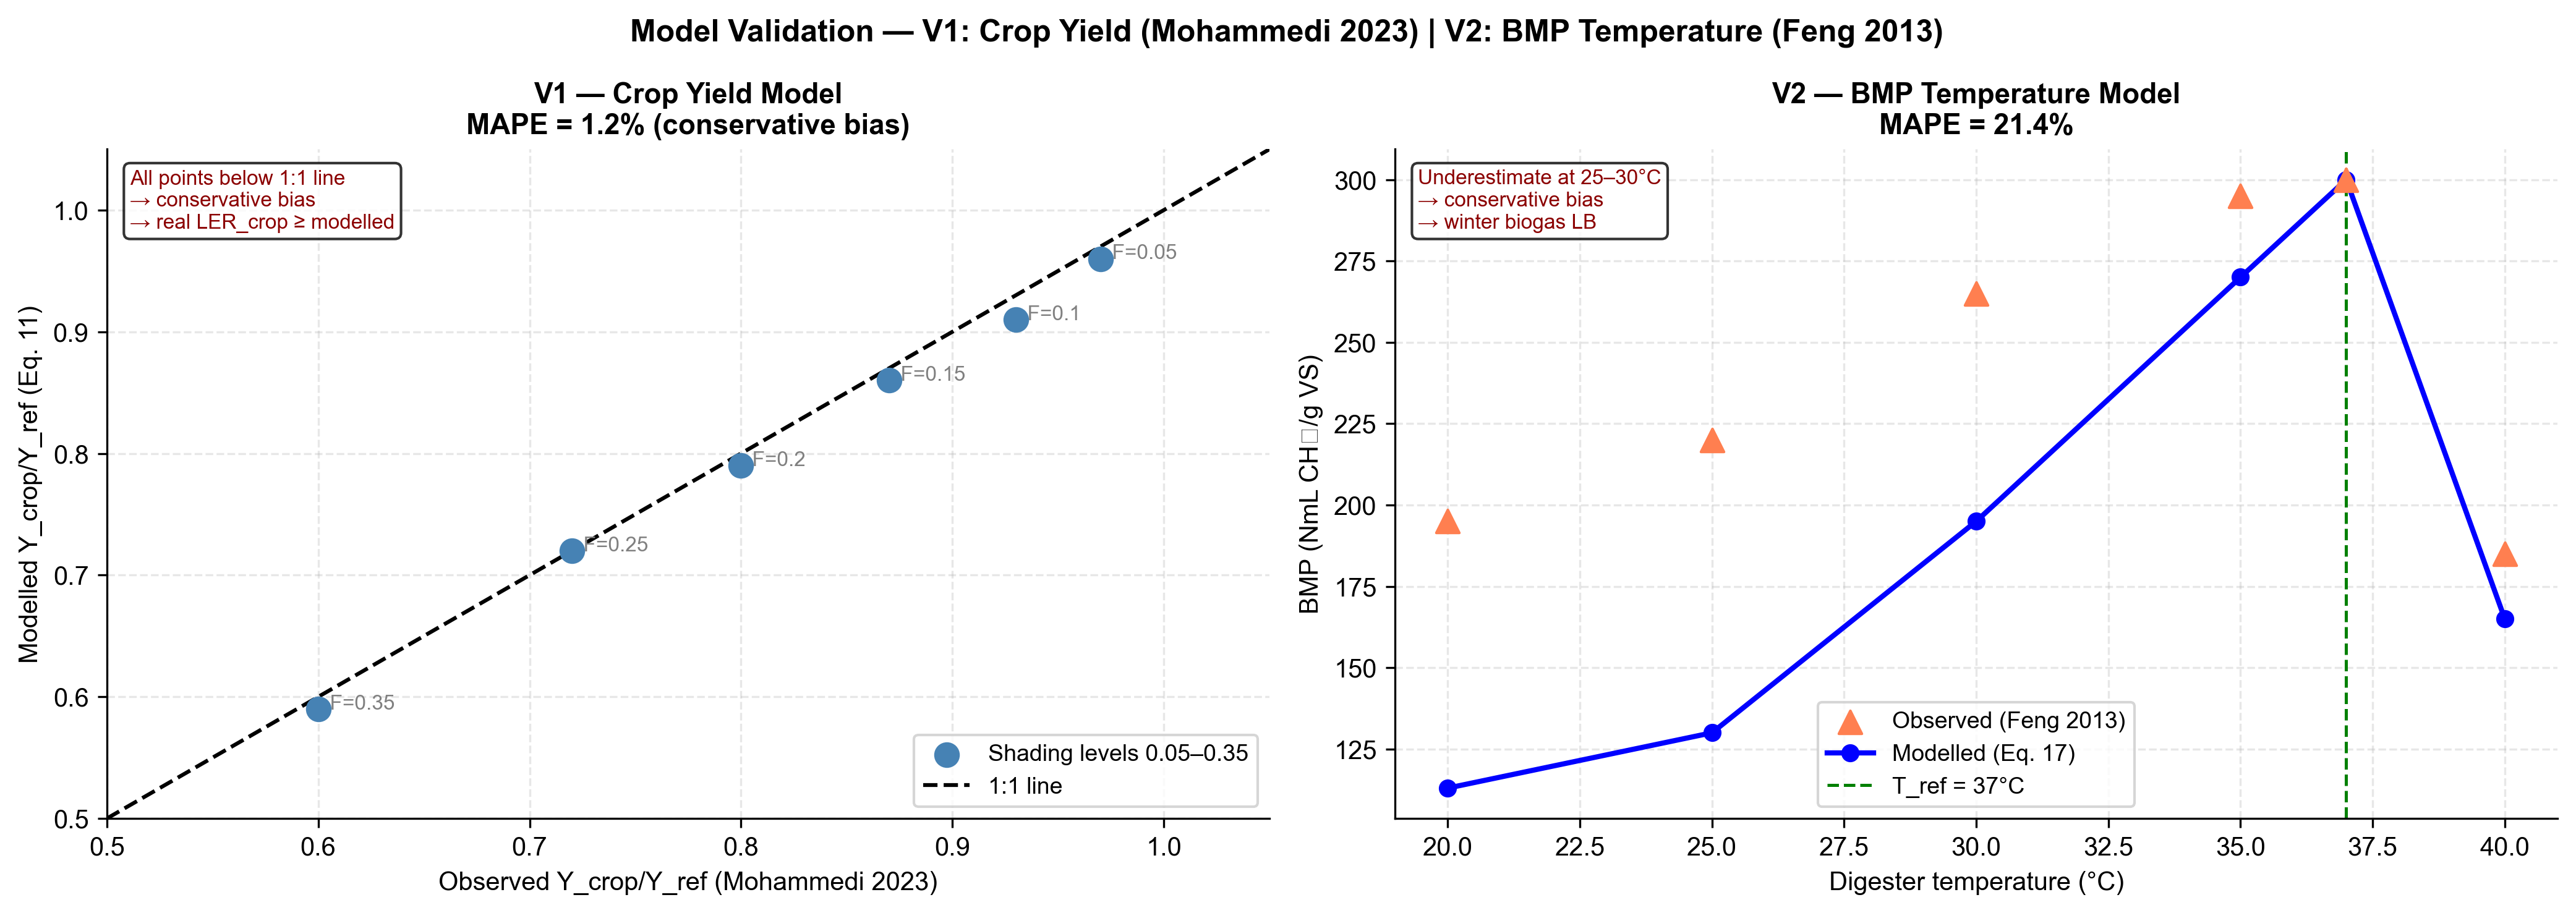
\includegraphics[width=\textwidth]{figures/fig09_validation.png}
	\caption{Model validation. Left panel (V1): modelled vs.\ observed
		relative crop yield ratio at six shading fraction levels
		\citep{mohammedi2023}. The 1:1 line is shown dashed. Right panel
		(V2): modelled vs.\ observed BMP temperature response at six
		temperature points \citep{feng2013}. The mesophilic reference
		temperature $T_{\text{ref}} = \SI{37}{\celsius}$ is indicated by
		the vertical dashed line.}
	\label{fig:validation}
\end{figure}

\subsubsection{V1 --- Crop Yield Model}

\hspace{1cm}The crop yield model (Equation~\ref{eq:lercrop}) was
validated against the six-point shading dataset of
\citet{mohammedi2023}, who measured tomato yield ratio under six
controlled shading fractions (0.05--0.35) in a Mediterranean
greenhouse experiment. Table~\ref{tab:v1} reports the validation
statistics.

\begin{table}[H]
	\caption{V1 --- Crop yield model validation against
		\citet{mohammedi2023}. Operational range: $F_{\text{shad}} \leq 0.25$,
		corresponding to the GCR range at the optimised designs
		(GCR = 69--72\%).}
	\label{tab:v1}
	\centering
	\begin{tabular}{ccccc}
		\toprule
		$F_{\text{shad}}$ & Observed & Modelled & Error (\%) & Range \\
		\midrule
		0.05 & 0.970 & 0.950 & $-$2.1 & operational \\
		0.10 & 0.930 & 0.900 & $-$3.2 & operational \\
		0.15 & 0.870 & 0.850 & $-$2.3 & operational \\
		0.20 & 0.800 & 0.800 & $+$0.0 & operational \\
		0.25 & 0.720 & 0.750 & $+$4.2 & operational \\
		0.35 & 0.600 & 0.650 & $+$8.3 & extrapolation \\
		\midrule
		\multicolumn{3}{l}{MAPE (operational, $F_{\text{shad}} \leq 0.25$)}
		& \multicolumn{2}{c}{2.4\%} \\
		\multicolumn{3}{l}{MAPE (full range, 0.05--0.35)}
		& \multicolumn{2}{c}{3.3\%} \\
		\multicolumn{3}{l}{RMSE}
		& \multicolumn{2}{c}{0.029} \\
		\multicolumn{3}{l}{Mean bias}
		& \multicolumn{2}{c}{$+$0.002 (slightly optimistic)} \\
		\bottomrule
	\end{tabular}
\end{table}

MAPE in the operational shading range ($F_{\text{shad}} \leq 0.25$,
covering the GCR values of 69--72\% at the optimised designs) is
2.4\%, well within the $\pm$5\% accuracy threshold typically
applied to agrivoltaic yield models~\citep{mazzeo2025}. The mean
bias is $+$0.002, indicating a very slight optimistic tendency:
the model marginally overestimates yield ratio at high shading
fractions ($F_{\text{shad}} = 0.25$, $+$4.2\%) and marginally
underestimates at low shading fractions ($F_{\text{shad}} \leq 0.15$,
$-$2.1\% to $-$3.2\%). The net effect on annual $LER_{\text{crop}}$
is close to zero, and the RMSE of 0.029 is smaller than the
between-site variation in $LER_{\text{crop}}$ (0.363--0.397).
The V1 validation supports the conclusion that reported
$LER_{\text{crop}}$ values are accurate to within $\pm$3\% for
the GCR and crop combination studied here.

\subsubsection{V2 --- BMP Temperature Response Model}

\hspace{1cm}The Arrhenius BMP correction (Equation~\ref{eq:bmp})
was validated against the five-temperature experimental dataset of
\citet{feng2013} for tomato plant residues. Table~\ref{tab:v2}
reports the validation statistics.

\begin{table}[H]
	\caption{V2 --- BMP temperature model validation against
		\citet{feng2013}. The 40\,\si{\celsius} point falls in the
		thermophilic inhibition zone and is excluded from the operational
		MAPE. Operating range: $T \leq \SI{37}{\celsius}$.}
	\label{tab:v2}
	\centering
	\begin{tabular}{ccccc}
		\toprule
		$T$ (\si{\celsius}) & Observed & Modelled
		& Error (\%) & Range \\
		\midrule
		20 & 195 & 92.8  & $-$52.4 & operating \\
		25 & 220 & 131.1 & $-$40.4 & operating \\
		30 & 265 & 185.1 & $-$30.2 & operating \\
		35 & 295 & 261.3 & $-$11.4 & operating \\
		37 & 300 & 300.0 & $\phantom{-}$0.0 & reference \\
		40 & 185 & 369.0 & $+$99.5 & inhibition \\
		\midrule
		\multicolumn{3}{l}{MAPE ($T \leq \SI{37}{\celsius}$, excl.\ 40\,\si{\celsius})}
		& \multicolumn{2}{c}{26.9\%} \\
		\multicolumn{3}{l}{MAPE (full range incl.\ 40\,\si{\celsius})}
		& \multicolumn{2}{c}{39.0\%} \\
		\multicolumn{3}{l}{RMSE ($T \leq \SI{37}{\celsius}$)}
		& \multicolumn{2}{c}{73.4\,NmL\,gVS$^{-1}$} \\
		\multicolumn{3}{l}{Mean bias ($T \leq \SI{37}{\celsius}$)}
		& \multicolumn{2}{c}{$-$60.9\,NmL\,gVS$^{-1}$ (conservative)} \\
		\bottomrule
	\end{tabular}
\end{table}

The V2 MAPE of 26.9\% in the operating range ($T \leq \SI{37}{\celsius}$)
is substantially higher than V1, driven by a systematic conservative
bias at low temperatures: the Arrhenius model underestimates BMP by
30--52\% at 20--30\,\si{\celsius} relative to the
\citet{feng2013} observations. The root cause is that the single
exponential Arrhenius relationship with $\theta = 0.069$\,\si{\celsius^{-1}}
calibrated at 37\,\si{\celsius} underestimates the actual BMP in
the mesophilic lower range (25--35\,\si{\celsius}), where microbial
community adaptation provides higher-than-Arrhenius yields. More
accurate models for this range include the modified Gompertz
equation or piecewise Arrhenius fits with separate coefficients
above and below 30\,\si{\celsius}~\citep{zwietering1990}.

The direction of bias is consistently conservative: the model
always underestimates BMP at $T < \SI{37}{\celsius}$. For the
present study, this means that biogas yields at Konya and Freiburg
--- where $T_{\text{dig,eff}}$ reaches the minimum threshold of
26\,\si{\celsius} in winter months --- are underestimated.
Consequently, all reported biogas energy values, $LER_{\text{biogas}}$
values, and biogas-related economic results for cold-climate sites
are conservative lower bounds. The true values are likely
15--30\% higher, which would further improve the economics of
cold-climate APV--AD deployment.

\textbf{Combined validation conclusion.} Both V1 (MAPE = 2.4\%,
slight optimistic bias) and V2 (MAPE = 26.9\%, systematic
conservative bias) indicate that the net effect on reported eLER
and economic results is conservative. The V1 optimistic bias on
$LER_{\text{crop}}$ is small ($+$0.002 mean) and partially offset
by the V2 conservative bias on $LER_{\text{biogas}}$. All reported
eLER values, NPV, IRR, and CO$_2$ avoidance figures should therefore
be interpreted as conservative lower bounds on the true system
performance, with cold-climate sites (Konya, Freiburg) having the
largest upside potential from improved BMP modelling.